\documentclass[areasetadvanced]{scrartcl}

\usepackage[utf8]{inputenc}
\usepackage[T2A]{fontenc}
\usepackage[english,russian]{babel}
\usepackage{xcolor}

\usepackage[footskip=1cm,left=25mm, right=15mm, top=20mm, bottom=20mm]{geometry}
\usepackage{setspace}
\usepackage{amsmath, amssymb} 
\usepackage{graphicx}
\usepackage{tikz}
\usetikzlibrary{arrows.meta}
\usepackage{float}
\usepackage{dashrule}
\usepackage{fancyhdr} 
\usepackage{hyperref} 
\usepackage{parskip}
\usepackage{textcomp, enumitem}
\usepackage{indentfirst}
\usepackage{graphicx}
\usepackage{algorithm}
\usepackage{xltabular}
\usepackage{xtab}
\usepackage{algpseudocode}
\usepackage{array} 
\usepackage{geometry}
\usepackage{afterpage}
\usepackage{minted}
\setcounter{secnumdepth}{3} 
\setcounter{tocdepth}{3}    
\usepackage{listings} 
\usepackage{booktabs}
\usepackage{paracol} % параллельные колонки (левая/правая)

\newcommand{\icon}[1]{\includegraphics[height=1.2em]{#1}}

\tikzstyle{block} = [rectangle, rounded corners, minimum width=3cm, minimum height=1cm, text centered, draw=black, fill=lightgray]

\setkomafont{sectioning}{\normalfont\bfseries} 
\setkomafont{section}{\normalfont\Large\bfseries}
\setkomafont{subsection}{\normalfont\large\bfseries}
\setkomafont{subsubsection}{\normalfont\large\bfseries}
\setkomafont{paragraph}{\normalfont\large\bfseries} 
\newcommand{\twosideheading}[2]{%
  \noindent
  \begin{minipage}[t]{0.5\textwidth}\raggedright\small #1\end{minipage}%
  \begin{minipage}[t]{0.5\textwidth}\raggedleft\Large\bfseries #2\end{minipage}\\[-0.2em]
  \hrule
  \vspace{0.8em}
}
\lstset{
  language=Haskell,
  basicstyle=\ttfamily\small,
  keywordstyle=\color{blue}\bfseries,
  stringstyle=\color{red},
  commentstyle=\color{green!70!black},
  numbers=left,
  numberstyle=\tiny,
  stepnumber=1,
  numbersep=10pt,
  showstringspaces=false,
  breaklines=true,
  frame=single
}

\lstdefinelanguage{Lua}{
    keywords={function, end, if, then, else, elseif, for, while, do, repeat, until, break, return, local, and, or, not, true, false, nil},
    keywordstyle=\color{blue}\bfseries,
    stringstyle=\color{red},
    commentstyle=\color{green!70!black},
    morestring=[s]{"}{"},
    morestring=[s]{'}{'},
    morecomment=[l]{--},
    morecomment=[s]{--[[}{]]},
    basicstyle=\ttfamily\small,
    numbers=left,
    numberstyle=\tiny,
    stepnumber=1,
    numbersep=10pt,
    showstringspaces=false,
    breaklines=true,
    frame=single
}

\lstdefinestyle{py}{
    language=Python,
    basicstyle=\ttfamily\small,
    keywordstyle=\color{blue}\bfseries,
    stringstyle=\color{red},
    commentstyle=\color{green!70!black},
    numbers=left,
    numberstyle=\tiny,
    stepnumber=1,
    numbersep=10pt,
    showstringspaces=false,
    breaklines=true,
    frame=single
}

\setlength{\parindent}{1.25cm}
\setcounter{tocdepth}{3}
\begin{document}
\sloppy
	\thispagestyle{empty}
	\begin{center}
		\large{МИНОБРНАУКИ РОССИИ} \par
		\vspace{0.3cm}
		\normalsize
		{ФЕДЕРАЛЬНОЕ ГОСУДАРСТВЕННОЕ АВТОНОМНОЕ ОБРАЗОВАТЕЛЬНОЕ УЧРЕЖДЕНИЕ ВЫСШЕГО ОБРАЗОВАНИЯ} \par
		\vspace{0.3cm}
		\textbf{\guillemotleft САНКТ-ПЕТЕРБУРГСКИЙ ПОЛИТЕХНИЧЕСКИЙ}
		\textbf{УНИВЕРСИТЕТ ПЕТРА ВЕЛИКОГО\guillemotright} \par
		\vspace{0.3cm}
		{Институт компьютерных наук и кибербезопасности}\par
		{Высшая школа технологий искусственного интеллекта}\par
	\end{center}
	\vfill
	\begin{center}
		{\huge Отчёт о выполнении лабораторных работ}\par
		%\vspace{0.1cm}
        \huge {по дисциплине:}\par
        \vspace{0.3cm}
		\Huge \textbf{Защита информации}\par
	\end{center}
	\vfill
	\begin{flushleft}
		Студент: \hspace{1.8cm} \rule[0pt]{2.5cm}{0.5pt}\hfill Салимли Айзек Мухтар Оглы\par
		\vspace{1.5cm}
		Преподаватель: \hspace{0.55cm} \rule[0pt]{2.5cm}{0.5pt}\hfill  Силиненко Александр Витальевич
	\end{flushleft}
	\vspace{0.5cm}
	\begin{flushright}
		\guillemotleft \rule[0pt]{0.8cm}{0.5pt}\guillemotright \rule[0pt]{2cm}{0.5pt} 20\rule[0pt]{0.5cm}{0.5pt} г.
	\end{flushright}
	\vfill
	\begin{center}
		Санкт-Петербург, 2026
	\end{center}

\newpage
\begin{center}
	\textbf{РЕФЕРАТ}\par
    \textbf{Объем отчета: N с., M табл., K источн., L прил.}
\end{center}


\textbf{Ключевые слова:} Защита информации, банк угроз, базовые вектора уязвимостей, $\dots$

Отчет содержит информацию о проделанной работе по дисциплине "защита информации", которая включала в себя N лабораторных работ.

\begin{itemize}
    \item Лабораторная работа №1: \begin{itemize}
        \item Знакомство со структурой раздела «Угрозы» банка данных угроз безопасности
              информации ФСТЭК РФ (далее – Банк угроз).
        \item Знакомство со структурой раздела «Уязвимости» Банка угроз.
        \item Поиск информации в разделе Уязвимости Банка угроз по заданным критериям.
    \end{itemize}
    \item $\dots$
\end{itemize}

\newpage

\section*{Термины и определения}
\addcontentsline{toc}{section}{Термины и определения}

В отчете применяют следующие термины с соответствующими определениями:

\begin{center}
\renewcommand{\arraystretch}{0.75}
\setlength{\tabcolsep}{3pt}
\begin{longtable}{>{\raggedright\arraybackslash}p{3.5cm}>{\raggedright\arraybackslash}p{9.5cm}}
\caption{Термины и определения} \\
\label{tab:terms} \\
\toprule
\textbf{Термин} & \textbf{Определение} \\
\midrule
\endfirsthead
\caption[]{Термины и определения (продолжение)} \\
\toprule
\textbf{Термин} & \textbf{Определение} \\
\midrule
\endhead
\midrule
\multicolumn{2}{r}{Продолжение на следующей странице} \\
\endfoot
\bottomrule
\endlastfoot
Информация & Сведения о лицах, предметах, фактах, событиях, явлениях и процессах независимо от формы их представления. \\
\hline
Свойства Безопасности информации &  Конфиденциальность, Целостность, Доступность. \\
\hline
Угроза & Потенциально возможное событие, действие или фактор (внешний или внутренний), способный нарушить конфиденциальность, целостность или доступность данных, нанеся ущерб информационным системам или пользователям. \\
\hline
Риск & Критерий угрозы - вероятность реализации угрозы, использующей уязвимости информационных активов, что приводит к ущербу: нарушению конфиденциальности, целостности или доступности данных. \\
\hline
Банк угроз & официальный общедоступный ресурс, содержащий систематизированный перечень уязвимостей, угроз, способов их реализации и объектов воздействия в информационных системах. \\
\hline
ФСТЭК & Федеральная служба по техническому и экспортному контролю. \\
\hline
Программное обеспечение & Совокупность программ, процедур, правил, документации и данных, необходимых для функционирования систем обработки информации. \\
\hline
Операционная система & Совокупность программ, обеспечивающих управление ресурсами ЭВМ и взаимодействие пользователя с машиной. \\
\hline
CWE (Common Weakness Enumeration) & Международная система классификации недостатков, дефектов и уязвимостей в программном и аппаратном обеспечении \\
\hline
Наличие эксплойта & Специальная программа, фрагмент кода или последовательность команд, использующие уязвимости (ошибки, слабые места) в программном обеспечении (ПО) или операционных системах для проведения атаки.\\
\hline
CVSS 2.0 (Common Vulnerability Scoring System, v2.0) & Вторая версия открытого стандарта для оценки серьезности уязвимостей IT-систем \\
\hline
CVSS 3.0 (Common Vulnerability Scoring System, v3.0) & Третья версия открытого стандарта для оценки серьезности уязвимостей IT-систем \\
\end{longtable}
\end{center}

\newpage
\tableofcontents

\newpage
\section{Лабораторная работа №1}
\subsection*{Введение}
\addcontentsline{toc}{subsection}{Введение}

Анализ уязвимостей программного обеспечение (далее ПО) - процесс по выявлению недостатков ПО, которые могут
привести к нарушению безопасности информационной системы (см. Таб. \ref{tab:terms}).

Уязвимость представляет собой \guillemetleft слабое\guillemetright место в ПО, позволяющее злоумышленнику осуществить несанкционированный доступ, атаку или получить контроль над информацией.
Анализ уязвимостей направлен на предотвращение потенциальных угроз и устранение существующих проблем безопасности.

Целью лабораторной работы №1 - является получение навыков работы с банком угроз Федеральной службы по техническому и экспортному контролю (ФСТЭК России).

Банк угроз содержит информацию об уязвимостях ПО и методах их эксплуатации. В рамках работы необходимо изучить структуру Банка угроз 
и освоить поиск уязвимостей, для собственной операционной системы компьютера и операционной системы смартфона. 

\subsection{Раздел \guillemetleft Угрозы\guillemetright}

Раздел \guillemetleft Угрозы\guillemetright содержит информацию об аспектах, связанных с угрозами безопасности информации.
В нем представлена классификация угроз по их природе, воздействию и потенциальным последствиям.
Каждая угроза сопровождается подробным описанием методов атаки, целей и уязвимостей, используемых злоумышленниками.
Для оценки степени серьезности воздействия предусмотрен параметр уровня опасности.
Также раздел включает рекомендации по защите, позволяющие определить меры для предотвращения или минимизации угрозы.

В разделе можно фильтровать данные по: 
\begin{itemize}
    \item Контекстному поиску;
    \item По источнику угрозы;
    \item Последствиям реализации угрозы которые включают в себя пункты: \begin{itemize}
        \item Нарушение конфиденциальности;
        \item Нарушение целостности;
        \item Нарушение доступности.
    \end{itemize}
\end{itemize}

Ниже на рисунке \ref{fig:razdel_ugrozi}, представлен снимок экрана, раздела угроз:

\begin{figure}[H]
    \centering
    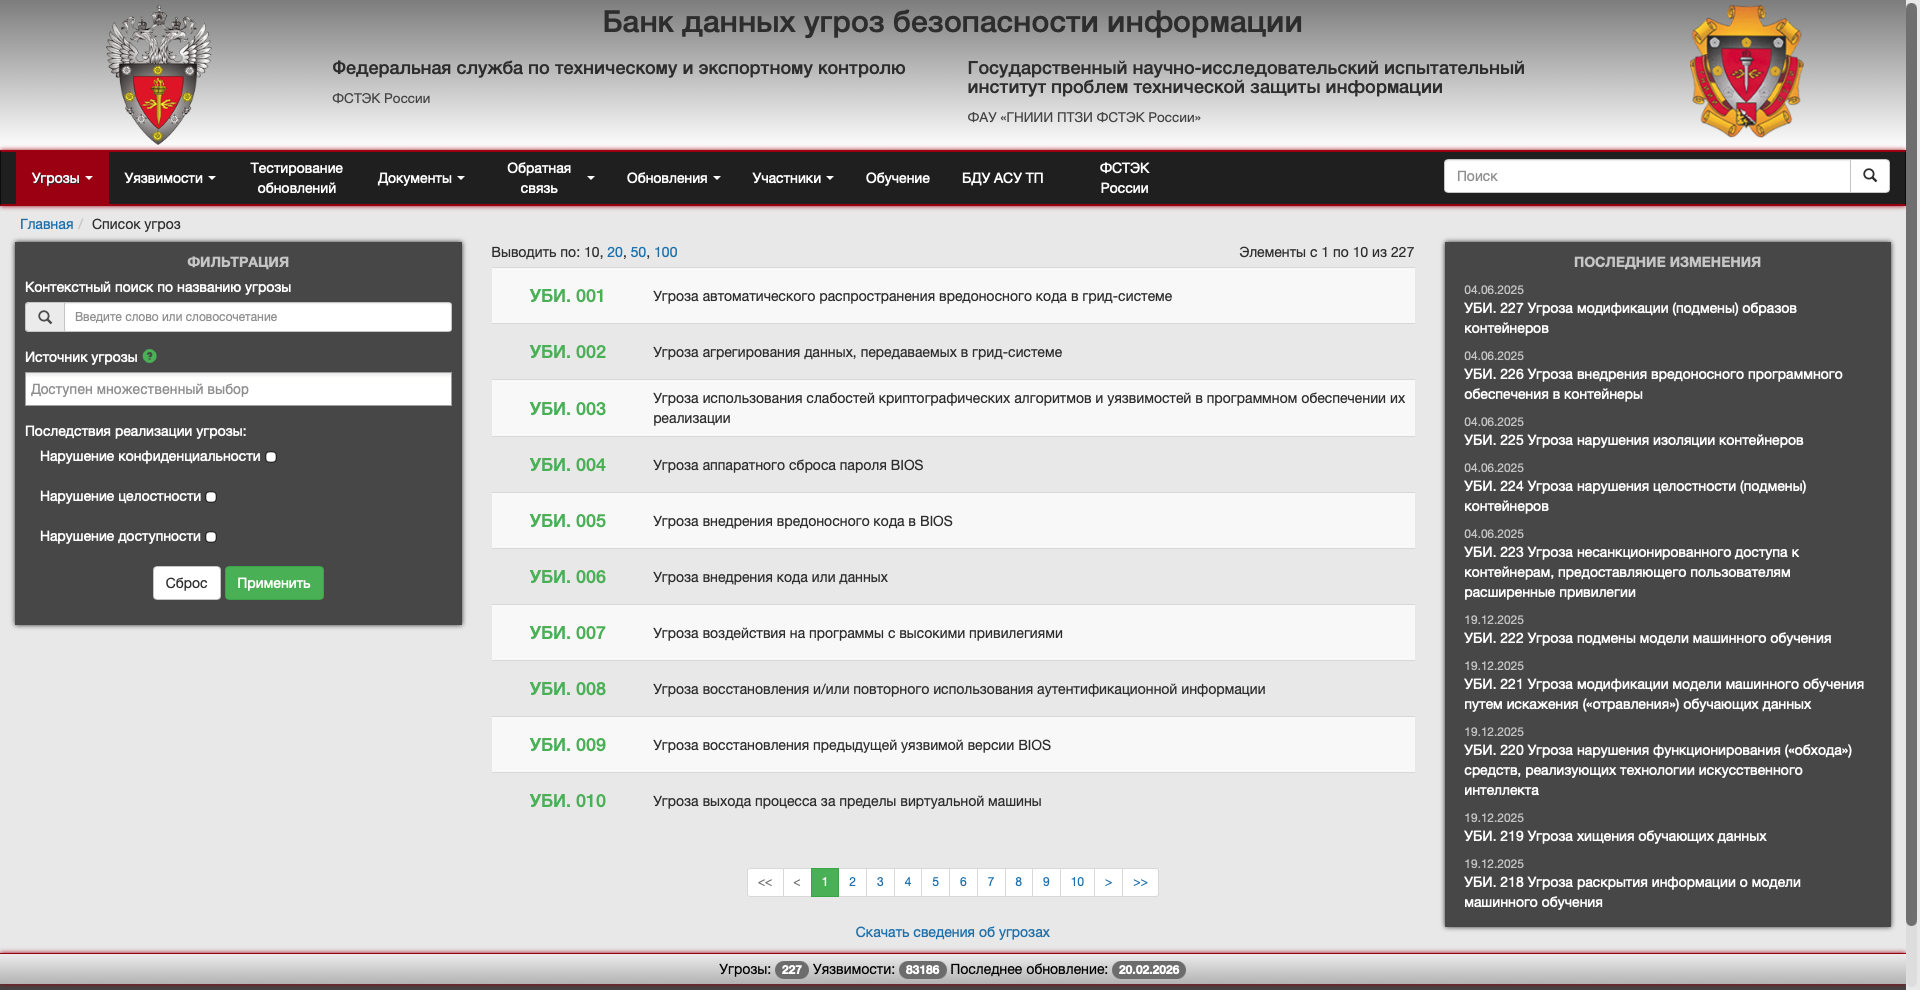
\includegraphics[width=0.60\linewidth]{img/RAZDEL_UGROZ.png}
    \caption{Раздел угроз}
    \label{fig:razdel_ugrozi}
\end{figure}

\subsection{Раздел \guillemetleft Уязвимости\guillemetright}

Раздел \guillemetleft Список уязвимостей\guillemetright, представляет перечень потенциальных недостатков или уязвимых точек в ПО, аппаратуре или в информационных системах
которые могут быть использованы злоумышленниками для нарушения свойств безопасности информации (см. Таб. \ref{tab:terms}).

Основным отличием уязвимости и угрозы - в том, что уязвимость это недостаток ПО (или системы), а угроза - это риск того что уязвимостью воспользуются.

То есть уязвимость существует сама по себе, а угроза существует условно.

Уязвимости делятся по определенным критериям:
\begin{itemize}
    \item Классификация уязвимости - отнесение уязвимости к конкретному классу, например в ФСТЭК классы делятся на: уязвимость кода, уязвимость арихтектуры и многофакторная;
    \item Год добавления - дата, когда уязвимасть была найдена и добавлена в банк угроз;
    \item Уровень опасности - делиться на 4 типа: Низкий, Средний, Высокий, Критический;
    \item Идентификатор типа ошибки - идентификатор, установленный в соответствии с общим перечнем ошибок CWE (см. Таб. \ref{tab:terms});
    \item Наличие эксплойта (см. Таб. \ref{tab:terms}) - Может существовать, быть в открытом доступе, не быть или уточняться;
    \item Способ эксплуатаци - какую именно угрозу несет уязвимость (например SQL-инъекция);
    \item Способ устранения - может быть обновление ПО или организационные меры;
    \item Операционная система - операционная система, под управлением которой функционирует программное обеспечение с обнаруженной уязвимостью.
\end{itemize} 

Наиболее опасная уязвимость - в ФСТЭК является возможность злоумышленника выполнять произвольные команды. 

Это можно увидеть, воспользовавшись сортировкой угроз (см. Рис. \ref{fig:SORT_BY_CRITICAL}) по уровню опасности (по критичности) описаной ранее:

\begin{figure}[H]
    \centering
    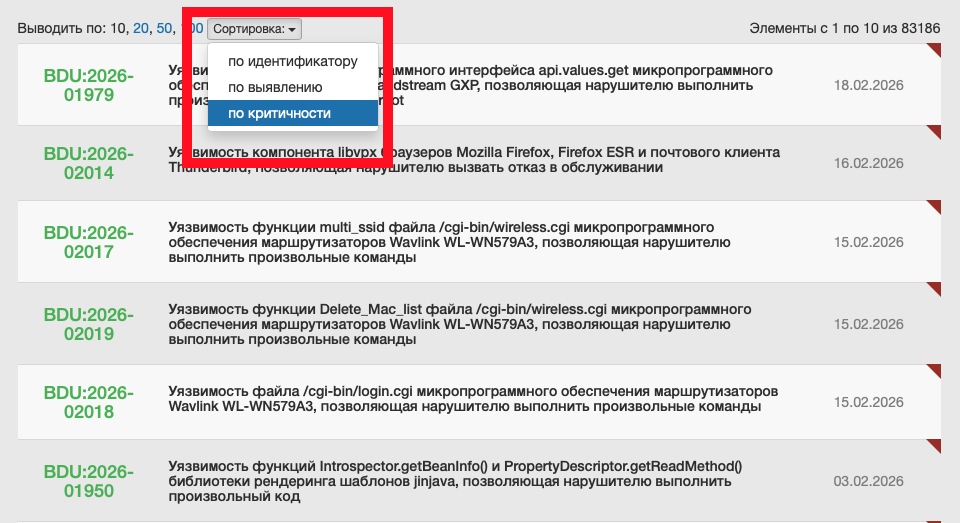
\includegraphics[width=0.60\linewidth]{img/SORT_BY_CRITICAL.png}
    \caption{Раздел угроз}
    \label{fig:SORT_BY_CRITICAL}
\end{figure}

Для визуального восприятия уязвимости так же помечаются цветом в соответствии с уровнем опасности:

\begin{itemize}
    \item \textcolor{green}{Низкий уровень опасности}
    \item \textcolor{yellow}{Средний уровень опасности}
    \item \textcolor{orange}{Высокий уровень опасности}
    \item \textcolor{red}{Критический уровень опасности}
\end{itemize}

Так же в разделе \guillemetleft Уязвимости\guillemetright, есть подраздел \guillemetleft Инфографика\guillemetright, 
который позволяет визуально оценить следующие данные:
\begin{itemize}
    \item Количество критических уязвимостей в ПО различных производителей (см. Рис \ref{fig:info_first})
    \item Распределение уязвимостей по уровням опасности (см. Рис \ref{fig:info_sec})
    \item Распределение уязвимостей по типам ПО (см. Рис \ref{fig:info_third})
    \item Количество уязвимостей в ПО различных производителей (см. Рис \ref{fig:info_fourth})
    \item Распределение уязвимостей по типам ошибок (см. Рис \ref{fig:info_fiveth})
    \item Количество уязвимостей программного обеспечения различных производителей, связанных с инцидентами информационной безопасности (см. Рис \ref{fig:info_sixth})
\end{itemize}

Ниже перечислены все инфографики описанные выше:

\begin{figure}[H]
    \centering
    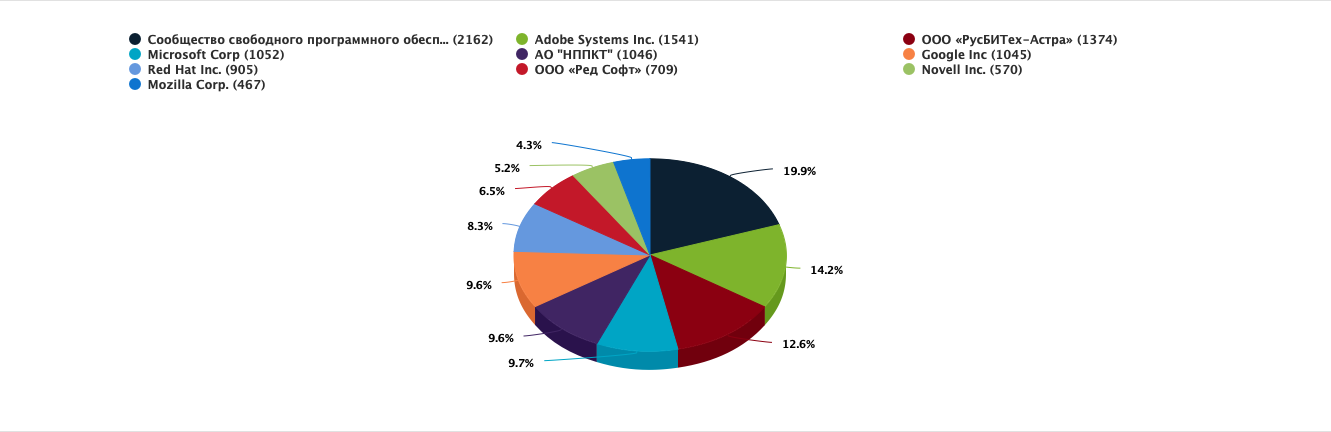
\includegraphics[width=0.60\linewidth]{img/info1.png}
    \caption{Количество критических уязвимостей в ПО различных производителей}
    \label{fig:info_first}
\end{figure}

Как видно из гистограммы \ref{fig:info_first}, количество критических уязвимостей больше наблюдается у сообщества 
свободного программного обеспечения. Вероятно это связано с тем, что это не большие компании, где нет отдельных специалистов обеспечивающих должную защиту информации.

\begin{figure}[H]
    \centering
    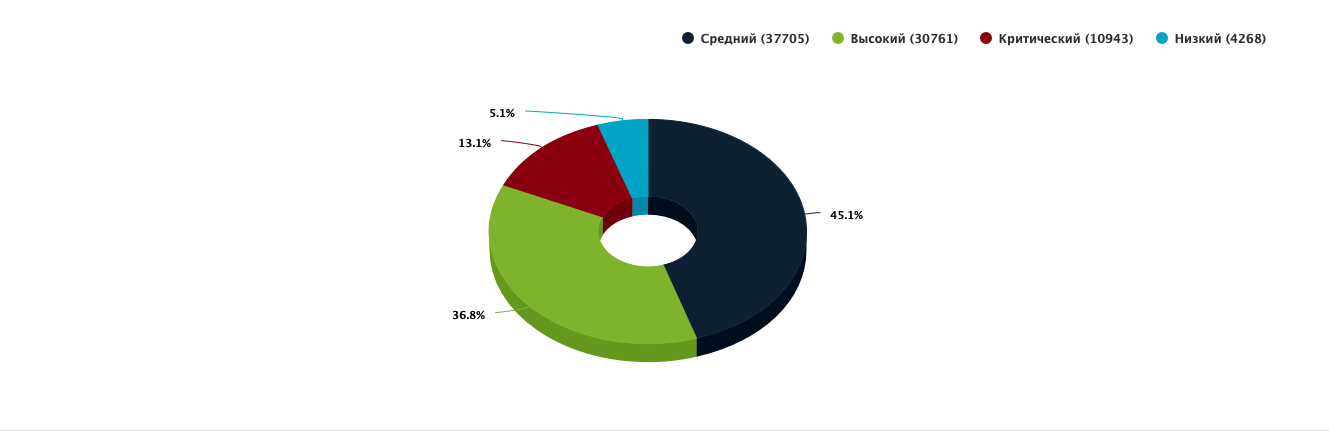
\includegraphics[width=0.60\linewidth]{img/info2.png}
    \caption{Распределение уязвимостей по уровням опасности}
    \label{fig:info_sec}
\end{figure}

Из рисунка \ref{fig:info_sec}, видно что больше всего уязвимостей имеют средний уровень опасности.

\begin{figure}[H]
    \centering
    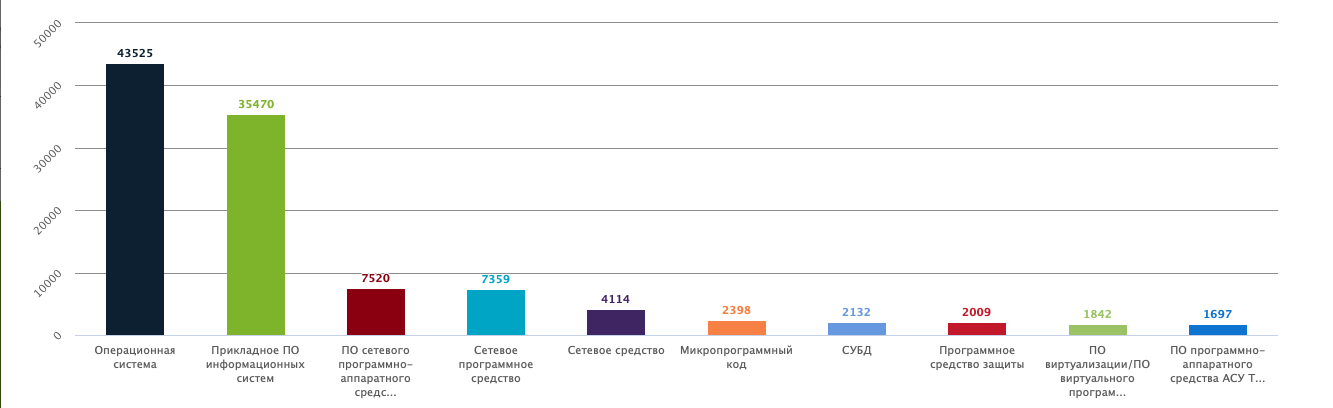
\includegraphics[width=0.60\linewidth]{img/info3.png}
    \caption{Распределение уязвимостей по типам ПО}
    \label{fig:info_third}
\end{figure}

Наиболее уязвимый тип ПО - является операционная система (см. Рис. \ref{fig:info_third}), что обусловлено тем, что ОС - довольно объемное и сложно программное обеспечение.

\begin{figure}[H]
    \centering
    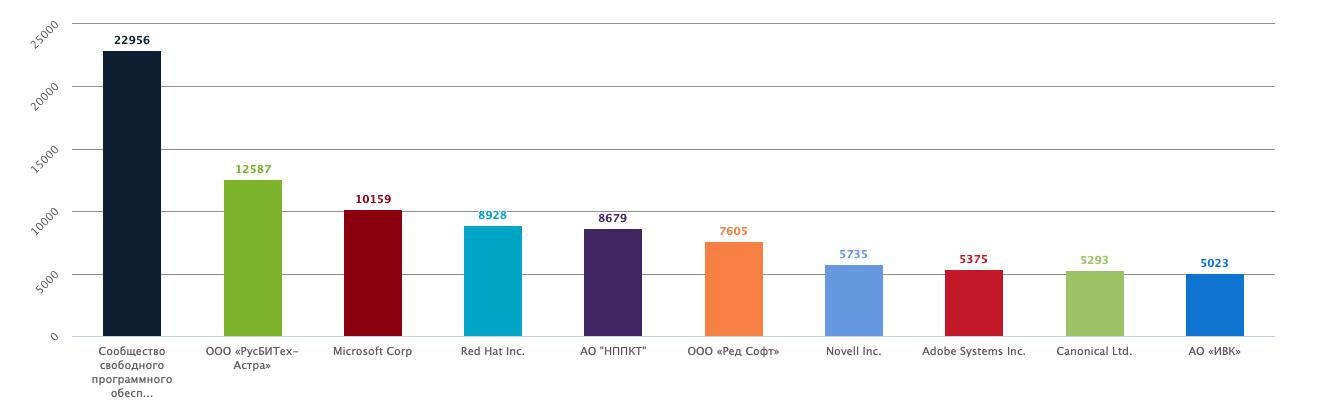
\includegraphics[width=0.60\linewidth]{img/info4.png}
    \caption{Количество уязвимостей в ПО различных производителей}
    \label{fig:info_fourth}
\end{figure}

Так же как и в случае с критическими уязвимостями (см. Рис. \ref{fig:info_first}), общее количество уязвимостей больше у сообщества свободного программного обеспечение (см. Рис. \ref{fig:info_fourth}).

\begin{figure}[H]
    \centering
    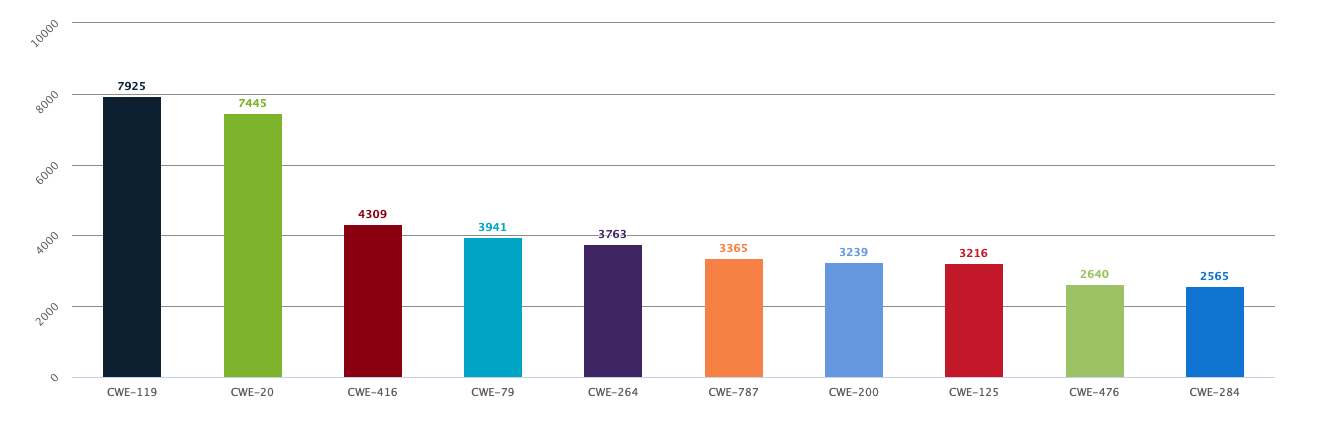
\includegraphics[width=0.60\linewidth]{img/info5.png}
    \caption{Распределение уязвимостей по типам ошибок}
    \label{fig:info_fiveth}
\end{figure}

Наиболее частая уязвимость по типу ошибки - CWE-119 (см. Рис. \ref{fig:info_fiveth}). CWE-119 - это ошибка связанная с неправильным ограничением операций в границах буфера памяти.

\begin{figure}[H]
    \centering
    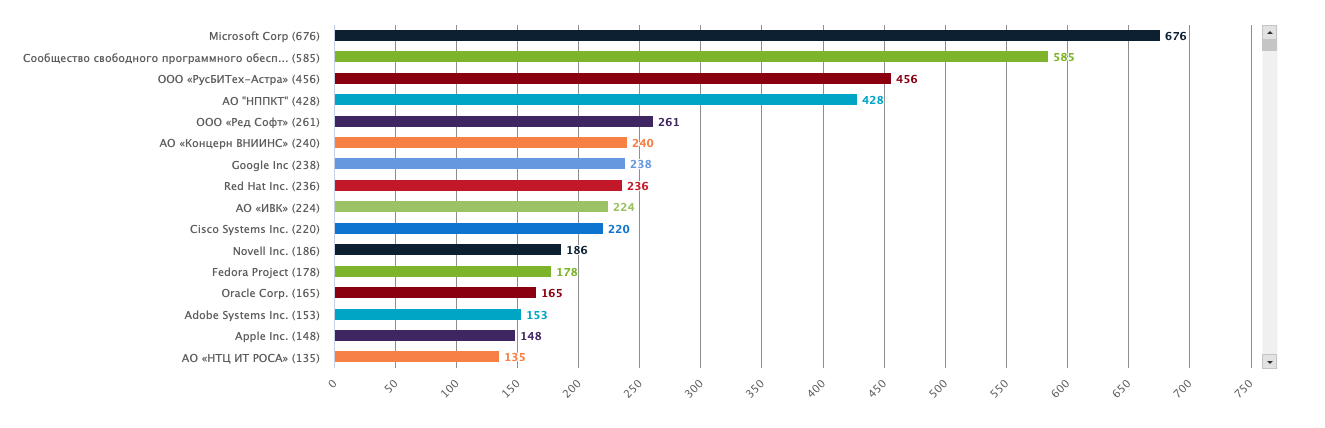
\includegraphics[width=0.60\linewidth]{img/info6.png}
    \caption{Количество уязвимостей ПО производителей, связанных с инцидентами ИБ}
    \label{fig:info_sixth}
\end{figure}

Из производителей, с наиболее частыми инцидентами в сфере ИБ является Microsoft Corp. На втором месте сообщество свободного программного обеспечения.

Из крупных производителей стоит так же отметить Google, который расположился на 7-ом месте, Apple inc. расположена на 15 месте. 

В списке так же присутствуют компании занимающиеся в основном разработкой дестрибутивов Linux. (См. Рис. \ref{fig:info_sixth}).

\subsection{Проверка собственной операционной системы}
В лабораторной работе №1, так же необходимо выполнить анализ уязвимостей операционной системы используемого ноутбука и смартфона.
\subsubsection{Описание аппаратного обеспечения}
В качестве используемых аппаратных средств:
\begin{enumerate}
\item Ноутбук: Apple MacBook Pro M3 Pro 18Gb/512Gb: \begin{itemize}
        \item Имя ОС: macOS Tahoe;
        \item Версионный индекс: 26.3 (25D125);
        \item Статус релиза: Стабильная;
        \item Ядро: Darwin Kernel Version 25.3.0;
        \item Архитектура: ARM64;
        \item Архитектура памяти: UMA.
    \end{itemize}
\item Смартфон: Apple iPhone 12 64Gb/4Gb: \begin{itemize}
        \item Имя ОС: iOS;
        \item Версионный индекс: 26.3 (23D127);
        \item Статус релиза: Стабильная.
    \end{itemize}
\end{enumerate}

Более подробная информация представлена на рисунке \ref{fig:macos}, для ноутбука и \ref{fig:ios}, для смартфона:

\begin{figure}[H]
    \centering
    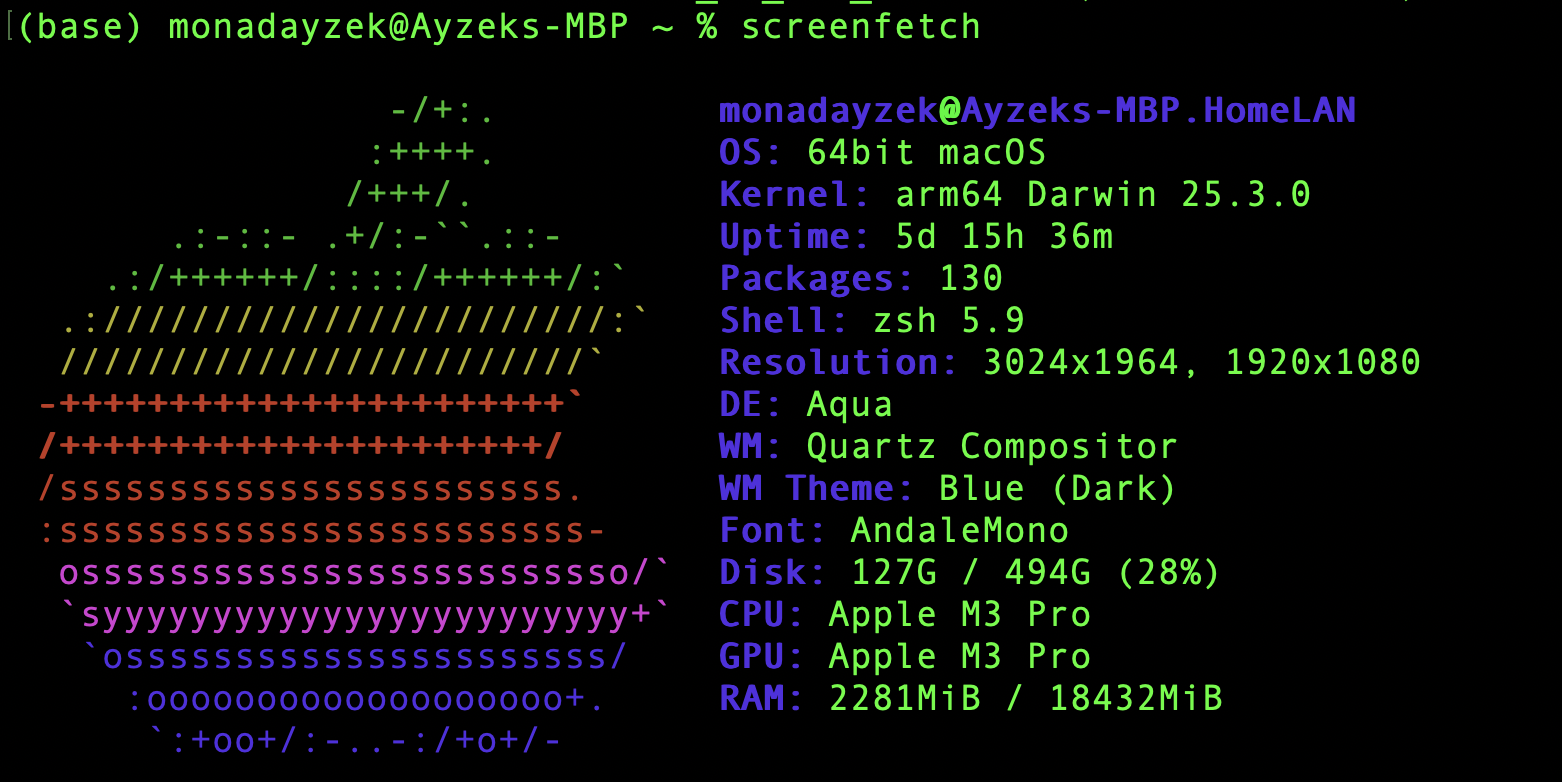
\includegraphics[width=0.60\linewidth]{img/macos.png}
    \caption{Информация об операционной системе (ноутбук)}
    \label{fig:macos}
\end{figure}

\begin{figure}[H]
    \centering
    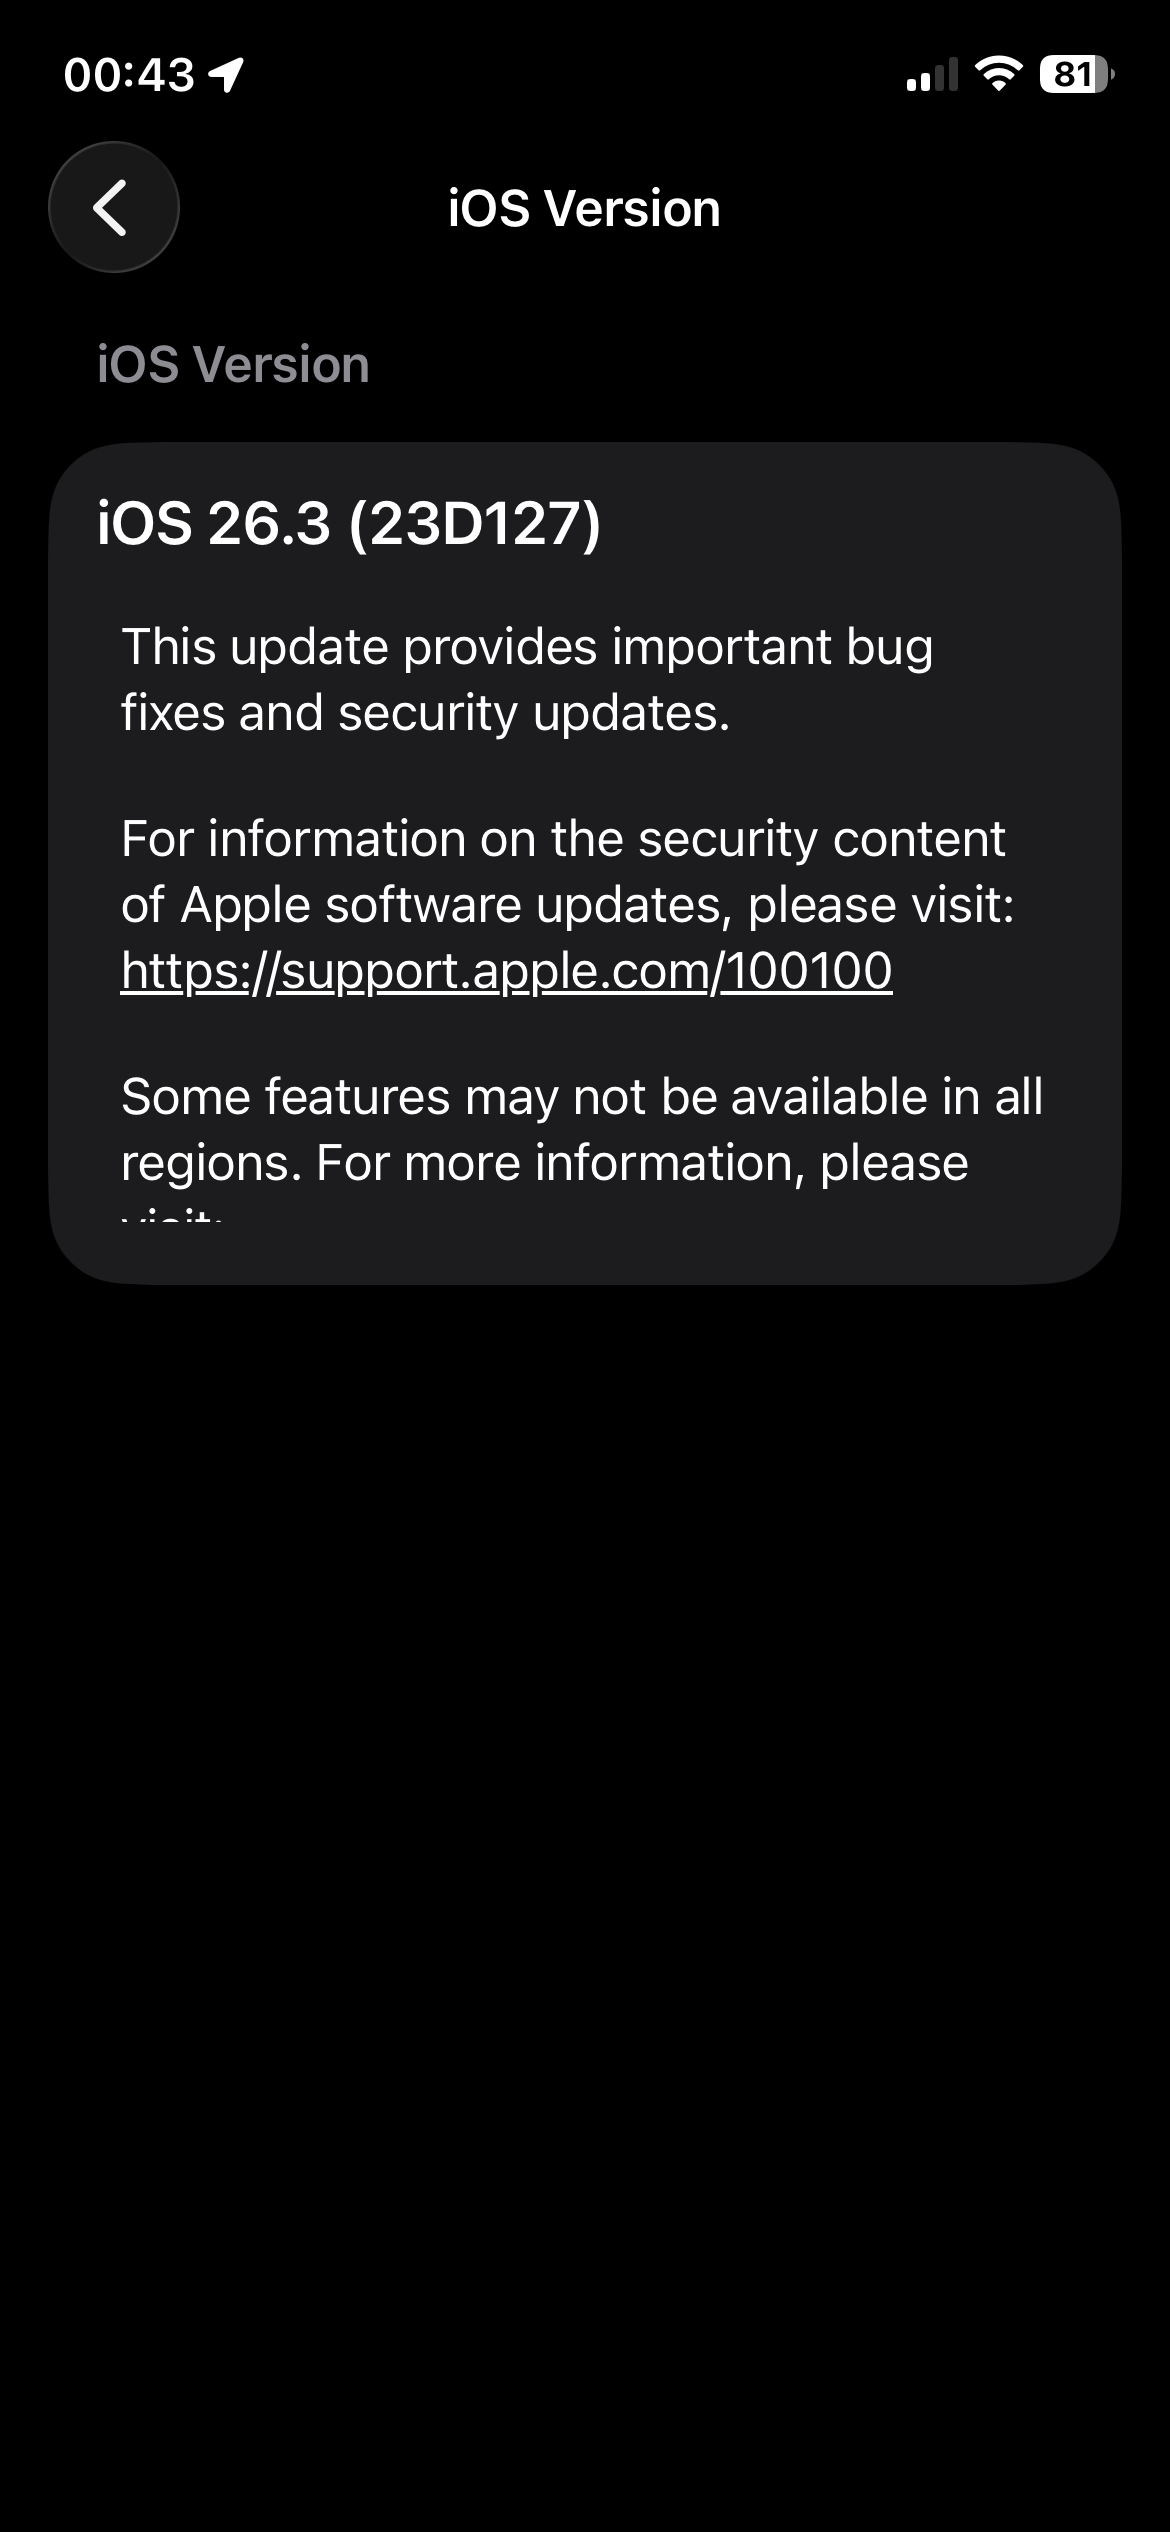
\includegraphics[width=0.28\linewidth]{img/ios.png}
    \caption{Информация об операционной системе (смартфон)}
    \label{fig:ios}
\end{figure}

\subsubsection{Поиск уязвимостей ОС ноутбука}
Для поиска уязвимостей операционной системы ноутбука, необходимо указать в поисковике слудющую информацию:
\begin{itemize}
    \item Производитель ПО: Apple;
    \item Тип ПО: Операционная система;
    \item Программное обеспечение: macOS;
    \item Аппаратная платформа: ARM64;
    \item Операционная система: MacOS Tahoe до 26.2 (крайняя версия ФСТЭК);
    \item Уровень опасности$^*$: Критический.
\end{itemize}

* - По поставленновки задачи лабораторной работы №1, требуется выявить \textcolor{red}{критические} уязвимости ПО. 
Если \textcolor{red}{критические} уязвимости не найдены, ищуться уязвимости \textcolor{orange}{высокой} опасности, если нет \textcolor{orange}{высокой} опасности, \textcolor{yellow}{средние} иначе \textcolor{green}{низкие}.

Как видно из рисунка \ref{fig:fstecmacos}, выявлено лишь три уязвимостей, две из которых \textcolor{yellow}{среднего} уровня, и одна \textcolor{green}{низкого} уровня.

\begin{figure}[H]
    \centering
    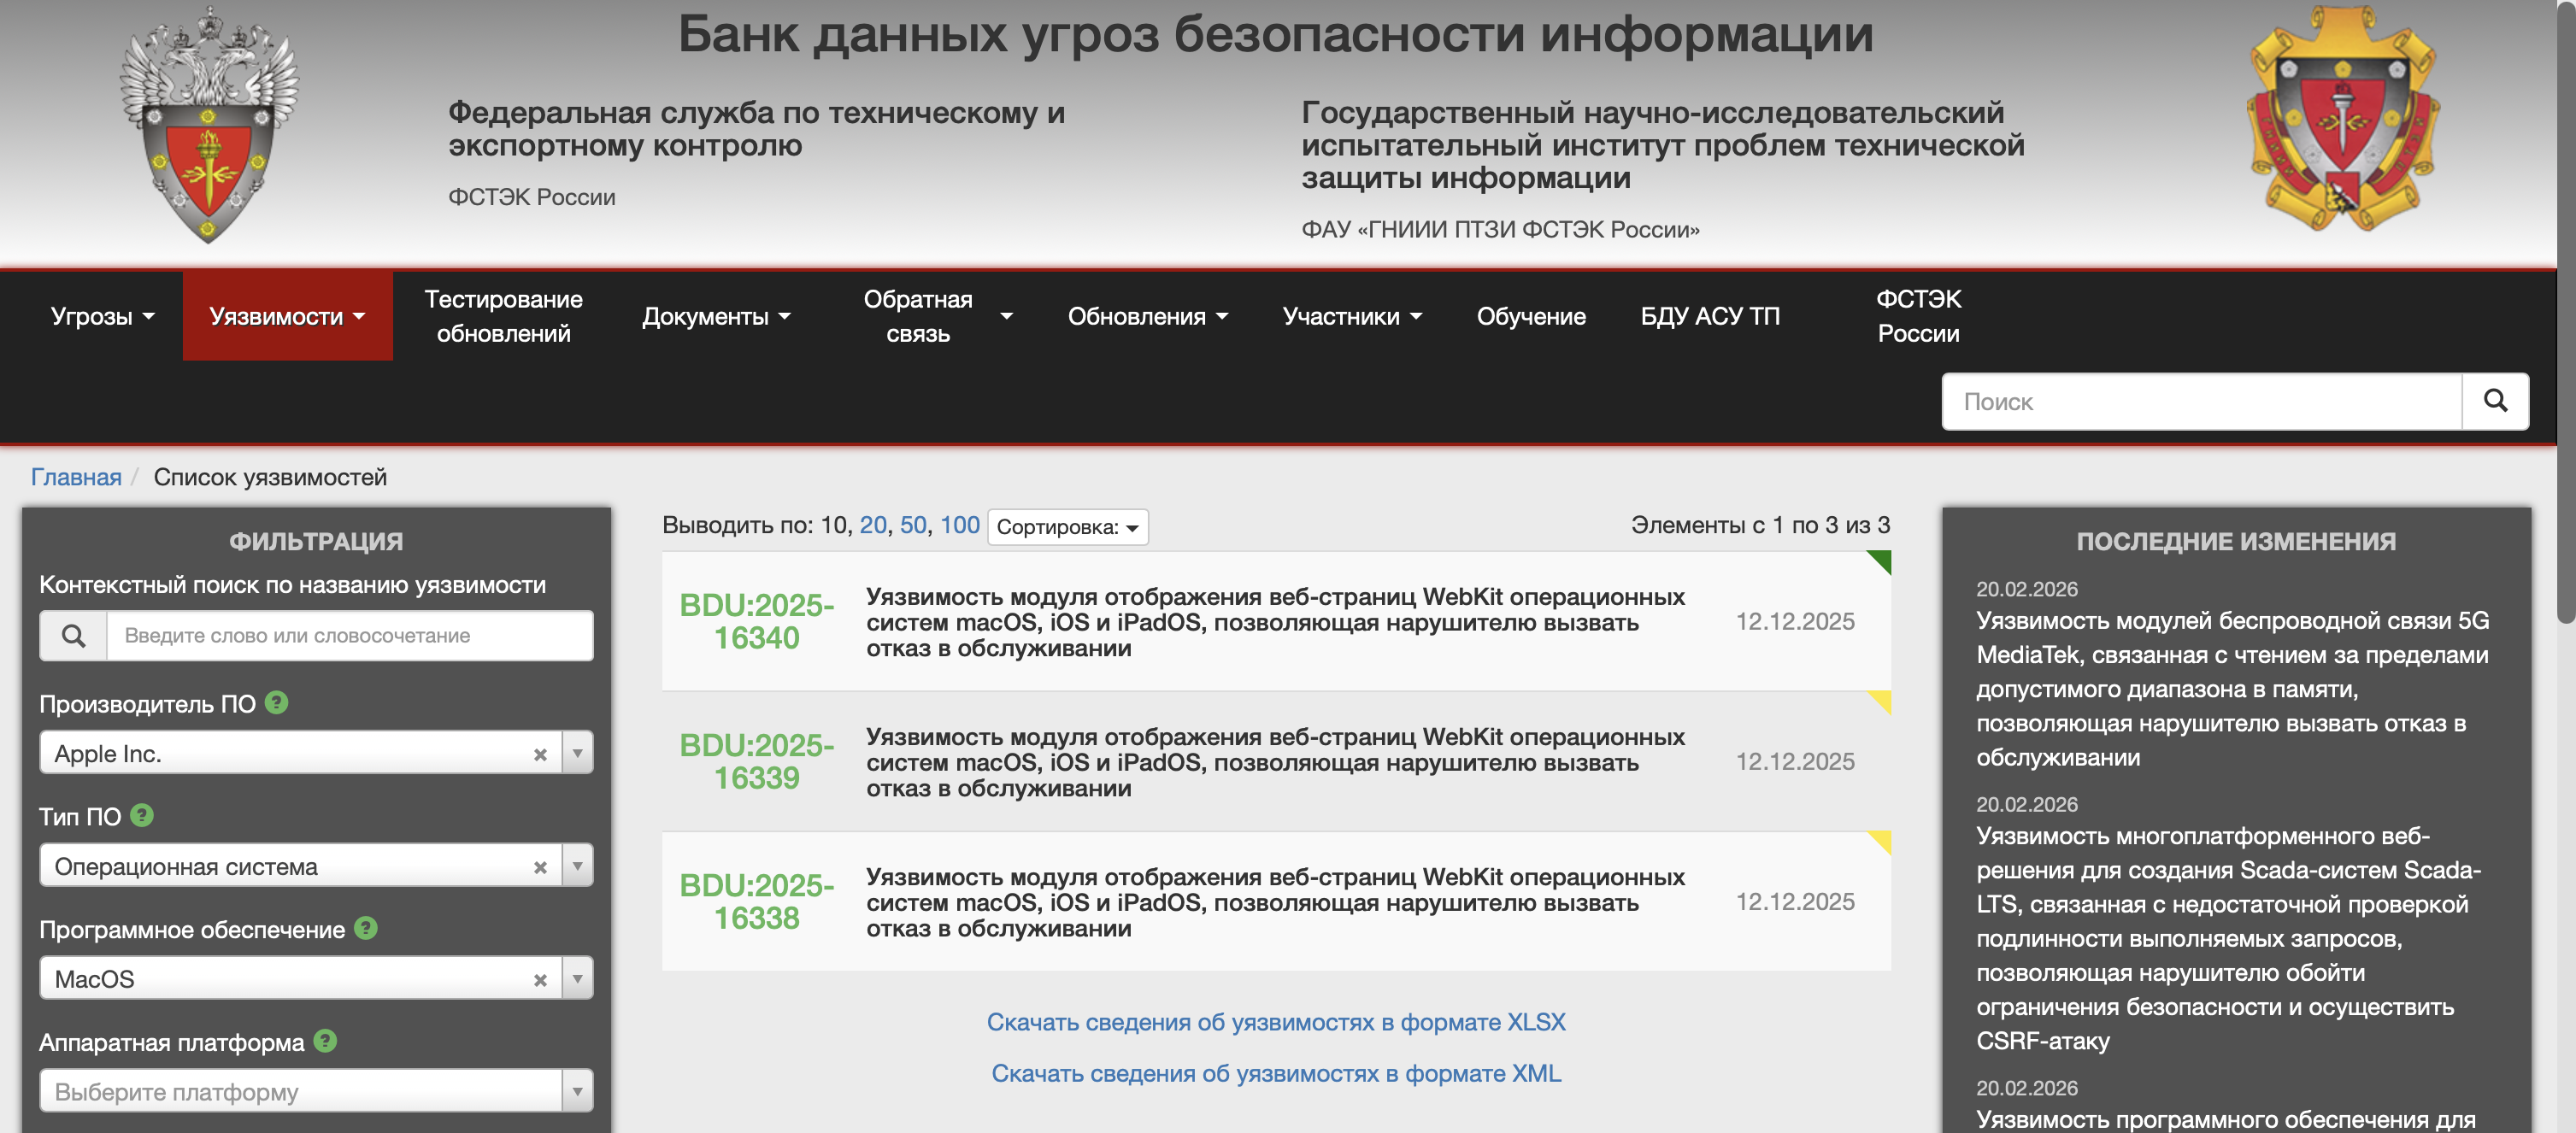
\includegraphics[width=0.60\linewidth]{img/fstecmacos.png}
    \caption{Уязвимости macOS 26.2}
    \label{fig:fstecmacos}
\end{figure}

Все уязвимости связанны с отображением страниц WebKit причем модули уязвимы как для macOS так и для iOS и iPadOS. 
Уязвимость позваляет злоумышленнику вызвать отказ в обслуживании. 

Более подробное описание двух средних уязвимостей представлено на рисунке \ref{fig:fstecmacos1full}, и \ref{fig:fstecmacos2full}, для низкого уровня на рисунке \ref{fig:fstecmacosfullgreen}.

\begin{figure}[H]
    \centering
    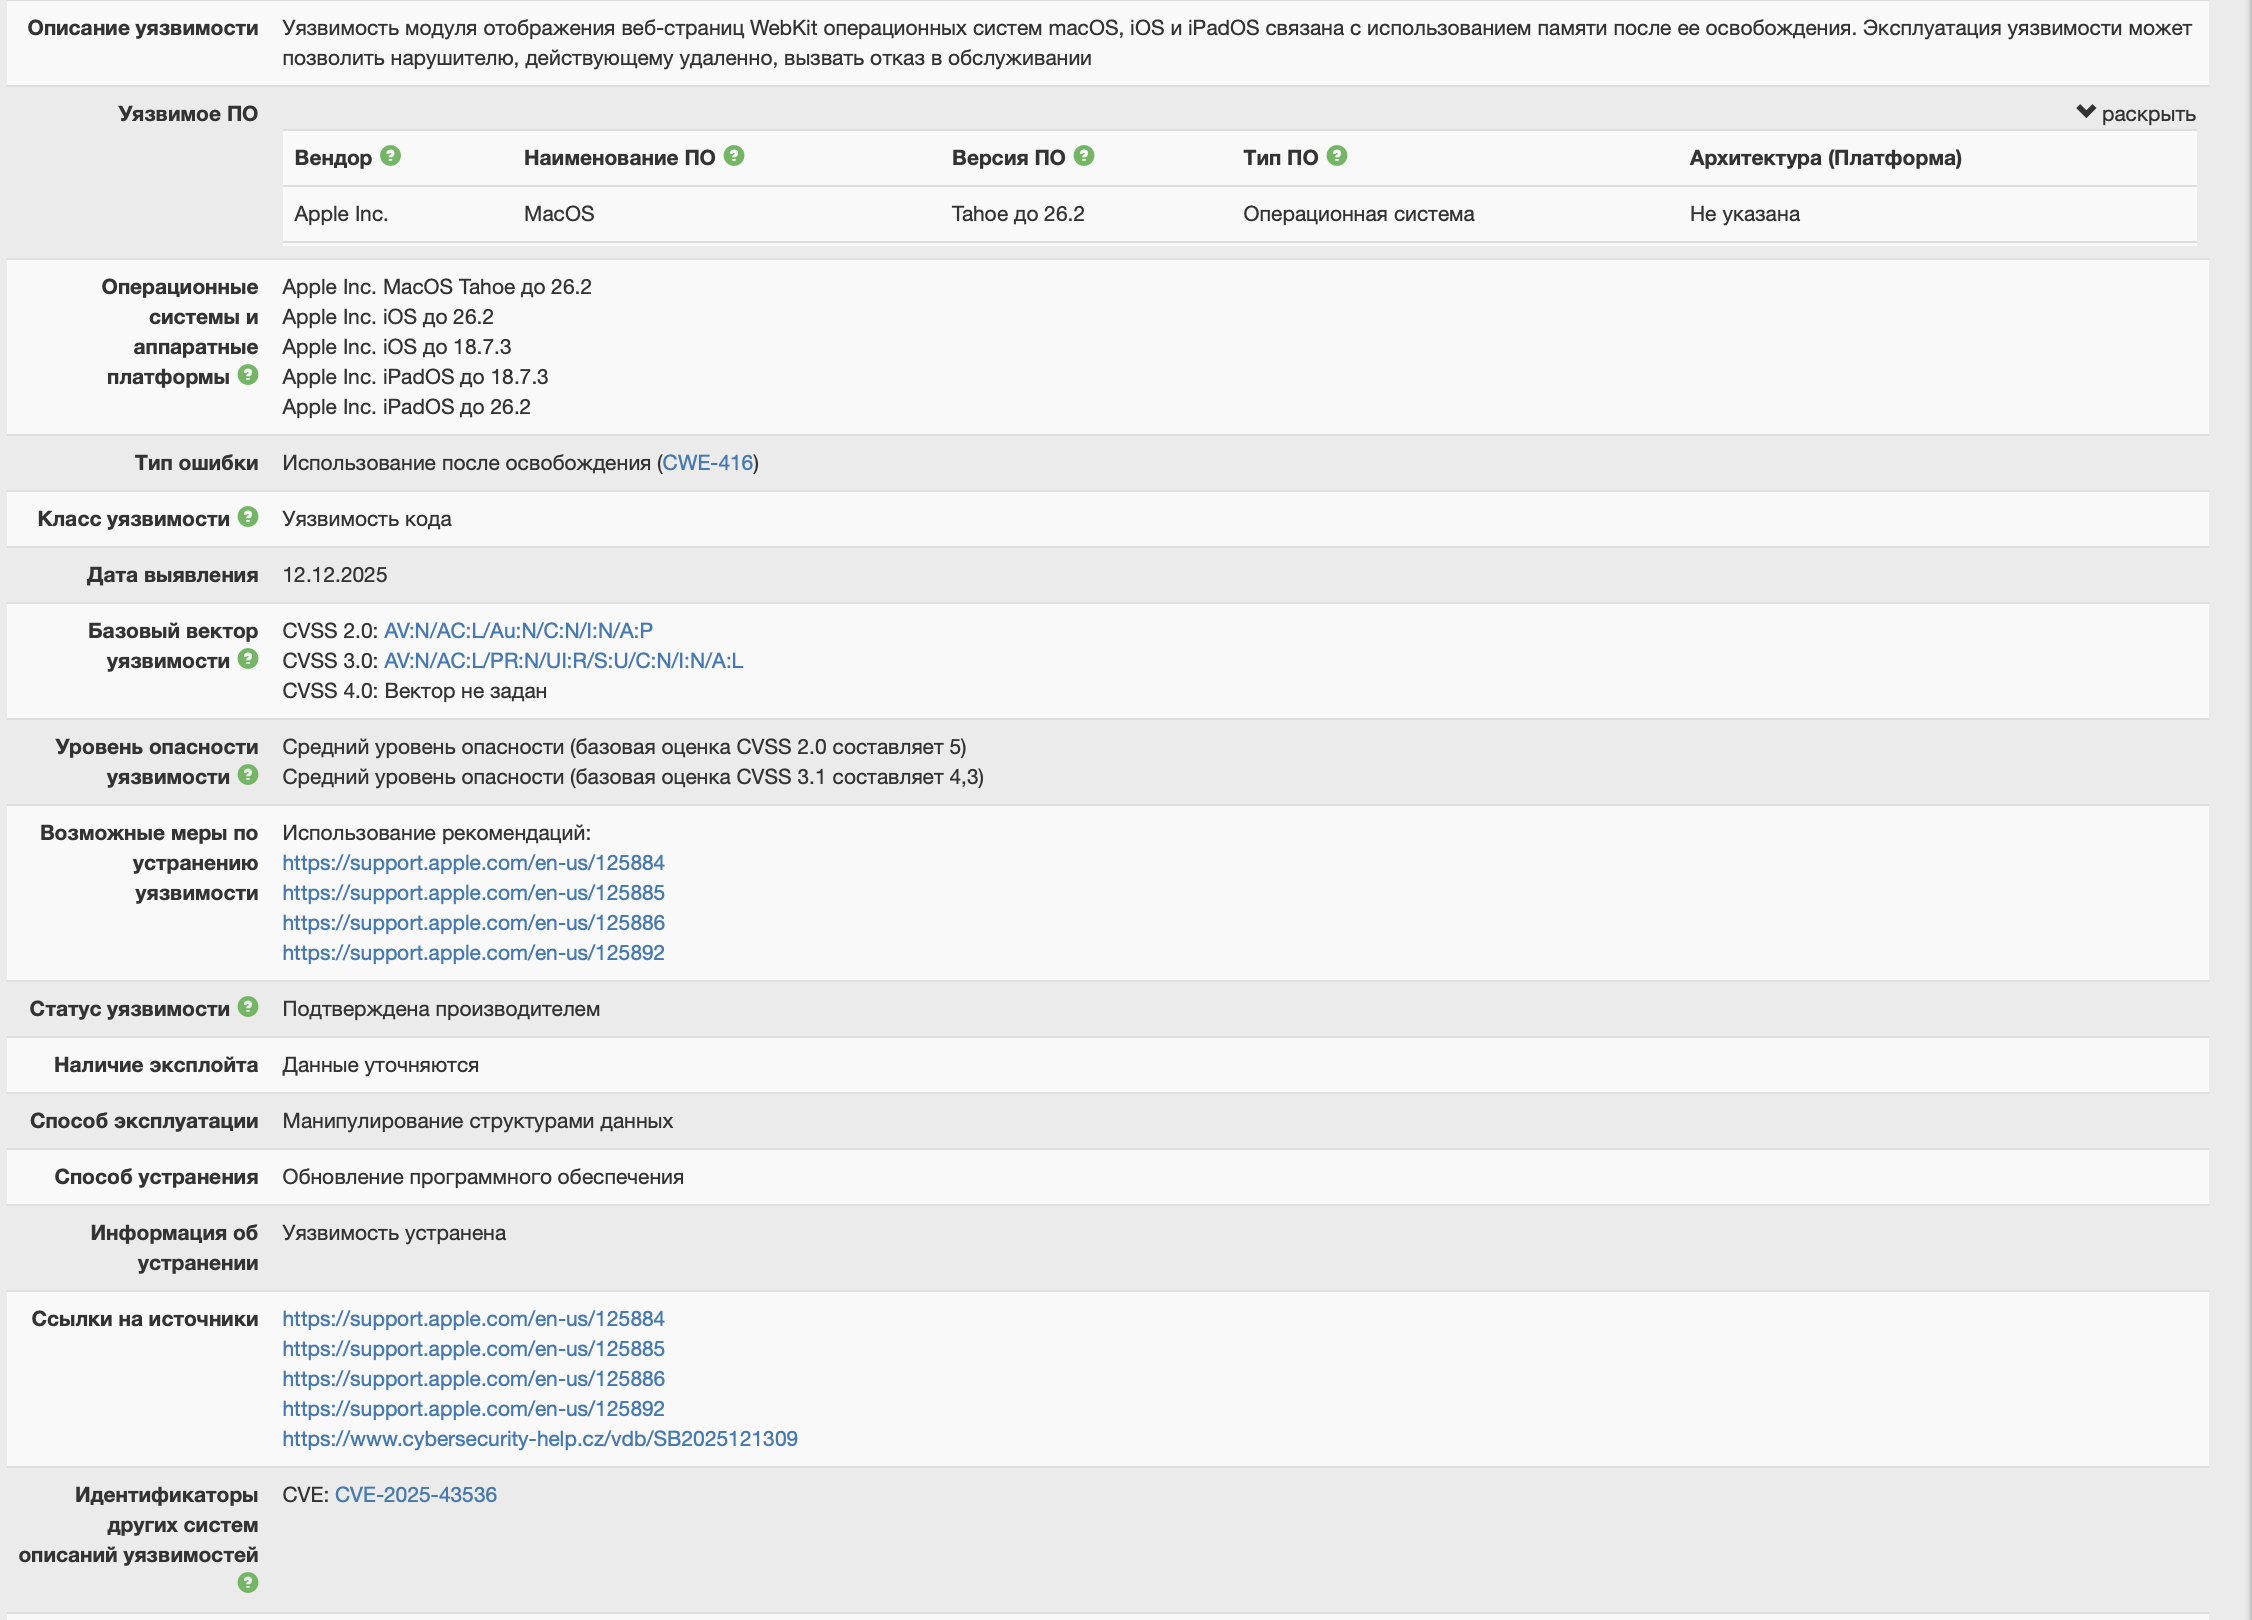
\includegraphics[width=0.60\linewidth]{img/fstecmacos2full.png}
    \caption{Уязвимость среднего уровня BDU:2025-16339}
    \label{fig:fstecmacos2full}
\end{figure}

\begin{figure}[H]
    \centering
    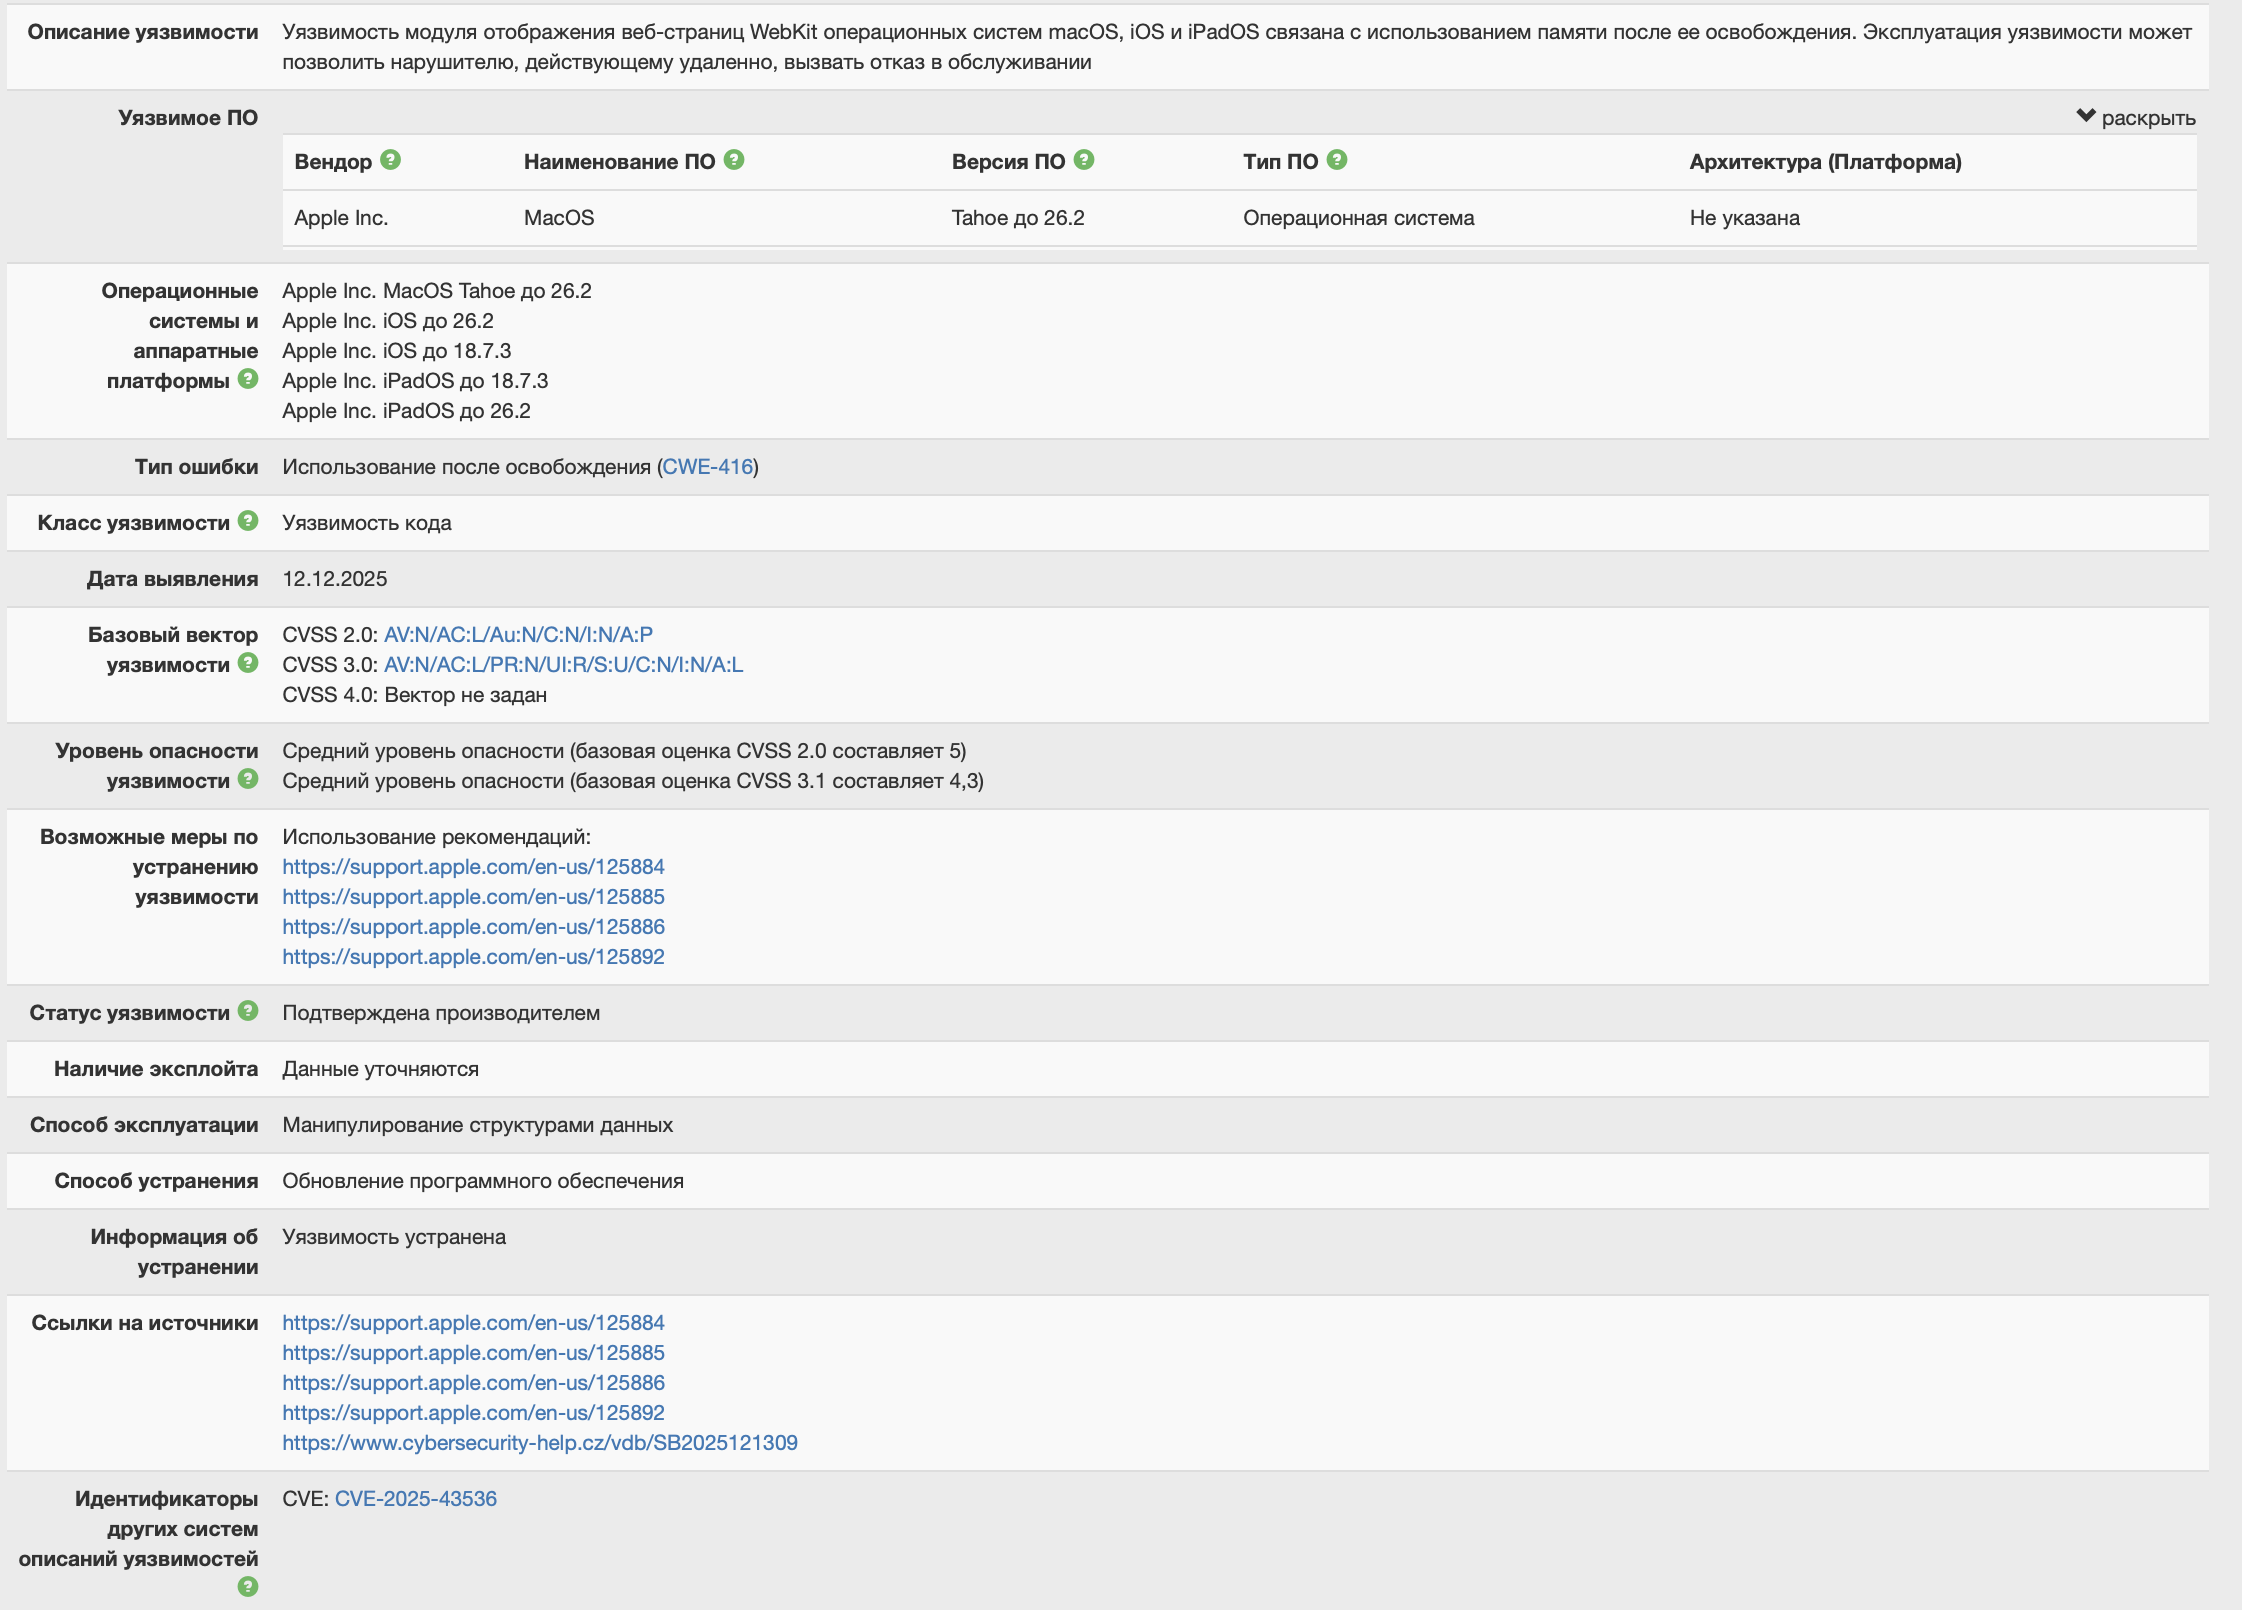
\includegraphics[width=0.60\linewidth]{img/fstecmacos1full.png}
    \caption{Уязвимость среднего уровня BDU:2025-16338}
    \label{fig:fstecmacos1full}
\end{figure}

\begin{figure}[H]
    \centering
    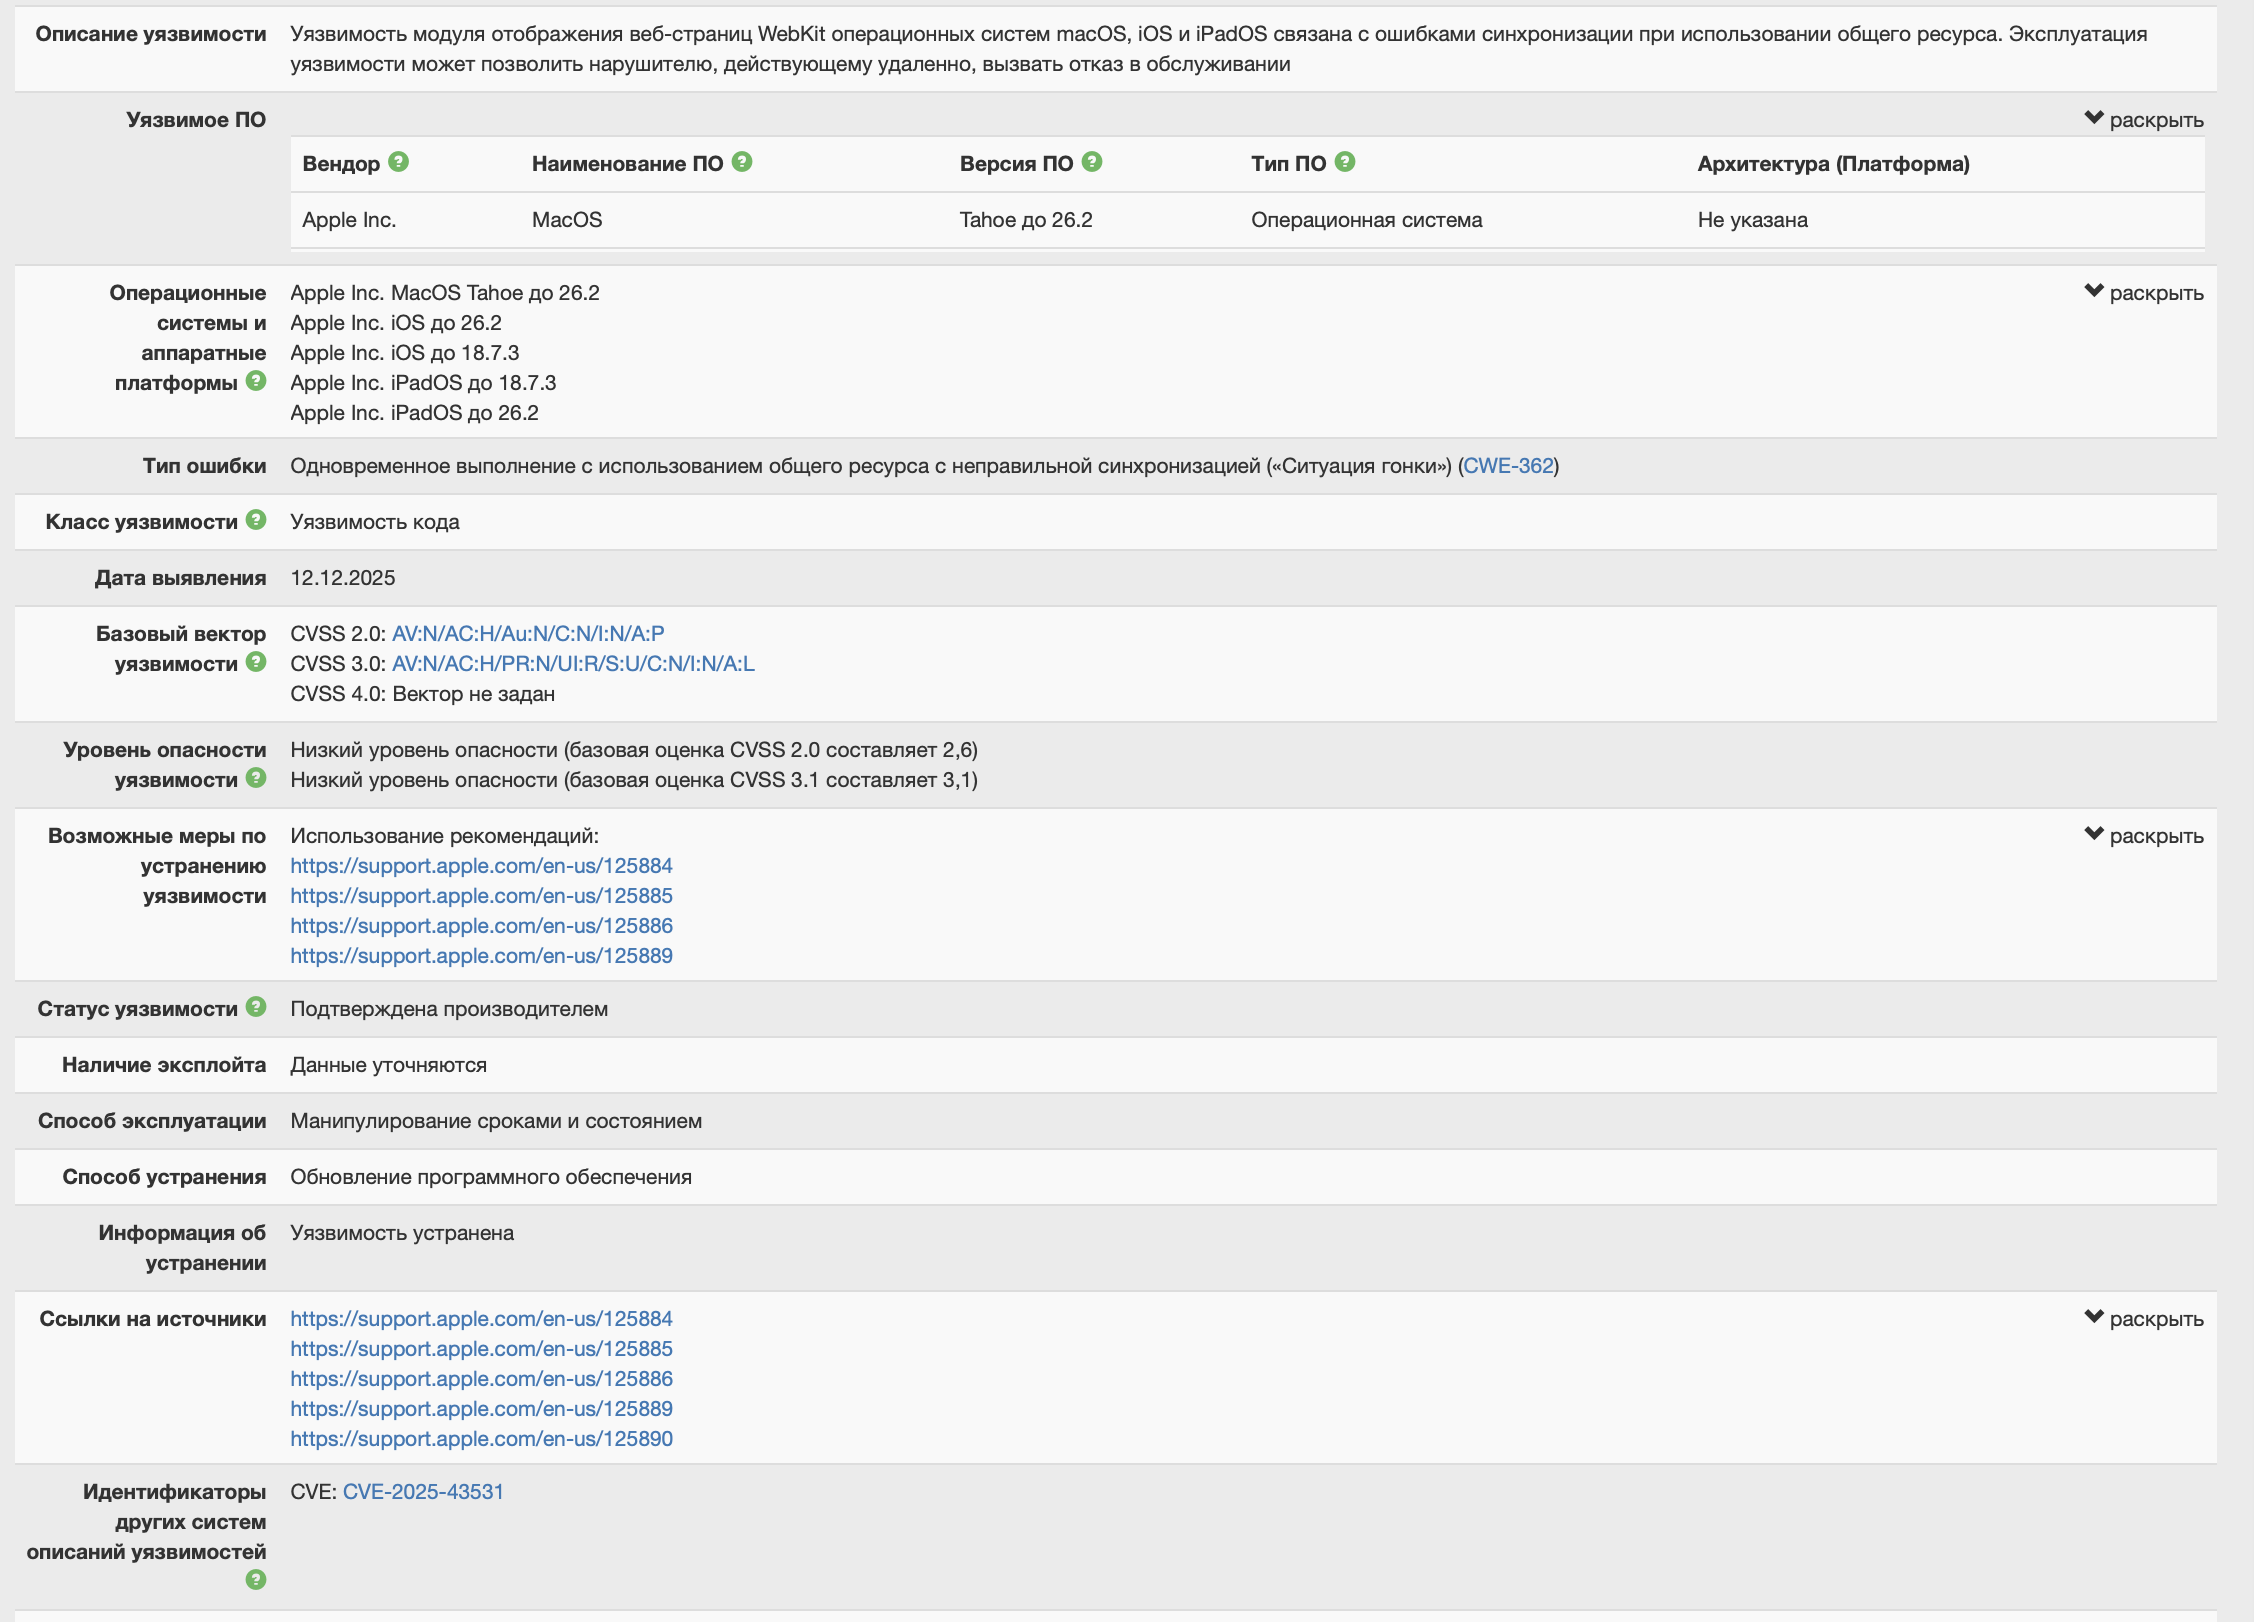
\includegraphics[width=0.60\linewidth]{img/fstecmacosfullgreen.png}
    \caption{Уязвимость низкого уровня BDU:2025-16340}
    \label{fig:fstecmacosfullgreen}
\end{figure}

Как видно, все три уязвимости относятся к типу уязвимости кода, и неотличимы друг от друга.

Ниже представленны таблица \ref{tab:cvss2}, и таблица \ref{tab:cvss3}, где перечислены все метрики векторов уязвимостей для CVSS 2.0 и CVSS 3.0 (см. Таб. \ref{tab:terms}) соответственно, с пояснением:

\begin{table}[H]
\centering
\small 
\caption{Метрики вектора уязвимости CVSS 2.0}
\label{tab:cvss2}
\begin{tabularx}{\textwidth}{|l|l|X|}
\hline
\textbf{Аббревиатура} & \textbf{Расшифровка} & \textbf{Значения и смысл} \\
\hline
AV  & Access Vector (вектор доступа) & \textbf{Local (L)} – локальный доступ; \textbf{Adjacent Network (A)} – доступ из смежной сети; \textbf{Network (N)} – сетевой доступ. Определяет способ взаимодействия с системой. \\
\hline
AC  & Access Complexity (сложность доступа) & \textbf{High (H)} – высокая; \textbf{Medium (M)} – средняя; \textbf{Low (L)} – низкая. Характеризует условия, необходимые для эксплуатации. \\
\hline
Au  & Authentication (аутентификация) & \textbf{Multiple (M)} – множественная; \textbf{Single (S)} – единственная; \textbf{None (N)} – не требуется. Указывает на необходимость подтверждения подлинности. \\
\hline
C   & Confidentiality Impact (влияние на конфиденциальность) & \textbf{None (N)} – отсутствует; \textbf{Partial (P)} – частичное; \textbf{Complete (C)} – полное. Степень раскрытия информации. \\
\hline
I   & Integrity Impact (влияние на целостность) & \textbf{None (N)} – отсутствует; \textbf{Partial (P)} – частичное; \textbf{Complete (C)} – полное. Возможность искажения данных. \\
\hline
A   & Availability Impact (влияние на доступность) & \textbf{None (N)} – отсутствует; \textbf{Partial (P)} – частичное; \textbf{Complete (C)} – полное. Степень нарушения доступности сервиса. \\
\hline
\end{tabularx}
\end{table}

\begin{table}[H]
\centering
\small
\caption{Метрики вектора уязвимости CVSS 3.0}
\label{tab:cvss3}
\begin{tabularx}{\textwidth}{|l|l|X|}
\hline
\textbf{Аббревиатура} & \textbf{Расшифровка} & \textbf{Значения и смысл} \\
\hline
AV  & Attack Vector (вектор атаки) & \textbf{Network (N)} – сетевой; \textbf{Adjacent (A)} – из смежной сети; \textbf{Local (L)} – локальный; \textbf{Physical (P)} – физический. Отражает удалённость атаки. \\
\hline
AC  & Attack Complexity (сложность атаки) & \textbf{Low (L)} – низкая; \textbf{High (H)} – высокая. Наличие условий вне контроля атакующего. \\
\hline
PR  & Privileges Required (необходимые привилегии) & \textbf{None (N)} – не требуются; \textbf{Low (L)} – низкие; \textbf{High (H)} – высокие. Уровень прав доступа до атаки. \\
\hline
UI  & User Interaction (взаимодействие с пользователем) & \textbf{None (N)} – не требуется; \textbf{Required (R)} – требуется. Участие другого лица в успешной атаке. \\
\hline
S   & Scope (область действия) & \textbf{Unchanged (U)} – не изменяется; \textbf{Changed (C)} – изменяется. Возможность воздействия на другие компоненты. \\
\hline
C   & Confidentiality Impact (влияние на конфиденциальность) & \textbf{High (H)} – высокое; \textbf{Low (L)} – низкое; \textbf{None (N)} – отсутствует. Степень потери конфиденциальности. \\
\hline
I   & Integrity Impact (влияние на целостность) & \textbf{High (H)} – высокое; \textbf{Low (L)} – низкое; \textbf{None (N)} – отсутствует. Возможность модификации данных. \\
\hline
A   & Availability Impact (влияние на доступность) & \textbf{High (H)} – высокое; \textbf{Low (L)} – низкое; \textbf{None (N)} – отсутствует. Степень нарушения доступности. \\
\hline
\end{tabularx}
\end{table}


Для более детального анализа, стоит расмотреть базойвый вектор уязвимости каждой уязвимости:

\begin{itemize}
    \item BDU:2025-16338: \begin{itemize}
        \item CVSS 2.0: AV:N/AC:L/Au:N/C:N/I:N/A:P (Оценка 5)
        \item CVSS 3.0: AV:N/AC:L/PR:N/UI:R/S:U/C:N/I:N/A:L (Оценка 4,3)
        \item CVSS 4.0: -
    \end{itemize} 
    \item BDU:2025-16339: \begin{itemize}
        \item CVSS 2.0: AV:N/AC:L/Au:N/C:N/I:N/A:P (Оценка 5)
        \item CVSS 3.0: AV:N/AC:L/PR:N/UI:R/S:U/C:N/I:N/A:L (Оценка 4,3)
        \item CVSS 4.0: -
    \end{itemize} 
    \item BDU:2025-16340: \begin{itemize}
        \item CVSS 2.0: AV:N/AC:H/Au:N/C:N/I:N/A:P (Оценка 2,6)
        \item CVSS 3.0: AV:N/AC:H/PR:N/UI:R/S:U/C:N/I:N/A:L (Оценка 3,1)
        \item CVSS 4.0: -
    \end{itemize} 
\end{itemize}

Так как вектора идентичны для средних уровней можно расписать их едино:

\textbf{CVSS 2.0: AV - способ получения доступа: N - сетевой/ AC - сложность получения доступа: L - низкая/ Au - аутентификация : N - не требуется/
C - влияние на конфиденциальность: N - не оказывает/ I - влияние на целостность: N - не оказывает/ A - влияние на доступность: P - частичное.}

\emph{Таким образом для CVSS 2.0, можно прочесть уязвимость как - сетевое подключение доступа с низкой сложнастью без аутентификации не влияющая на конфиденциальность не оказывающая влияние на целостность и частично влияющая на доступность.}

\textbf{CVSS 3.0: AV - Вектор атаки: N - сетевой/ AC - сложность атаки: L - низкая/ PR - уровень привелегий: N - не требуется/ UI - взаимодействие с пользователем: R - требуется/ S - влияние на другие компоненты системы: U - не оказывает/ C - влияние на конфиденциальность: N - не оказывает/ I - влияние на целостность: N - не оказыает/ A - влияние на доступность: L - низкое.}

\emph{Таким образом для CVSS 3.0, можно прочесть уязвимость как - сетевой вектор атаки с низкой сложностью, не требующий уровень привелегий с взаимодействием с пользователем, не влияющая на другие компоненты, не влияющая на конфиденциальность, без оказания влияния на целостность с низким влиянием на доступность.}

Вектор для низкого уровня уязвимости отличается лишь пунтом \guillemetleft сложность атаки\guillemetright (AC), и имеет индекст H, то есть высокая сложность. Таким образом для низкого уровня уязвимости:

\textbf{CVSS 2.0: AV - способ получения доступа: N - сетевой/ AC - сложность получения доступа: H - высокая/ Au - аутентификация : N - не требуется/
C - влияние на конфиденциальность: N - не оказывает/ I - влияние на целостность: N - не оказывает/ A - влияние на доступность: P - частичное.}

\emph{То есть - сетевое подключение доступа с высокой сложнастью без аутентификации не влияющая на конфиденциальность не оказывающая влияние на целостность и частично влияющая на доступность.}

\textbf{CVSS 3.0: AV - Вектор атаки: N - сетевой/ AC - сложность атаки: H - высокая/ PR - уровень привелегий: N - не требуется/ UI - взаимодействие с пользователем: R - требуется/ S - влияние на другие компоненты системы: U - не оказывает/ C - влияние на конфиденциальность: N - не оказывает/ I - влияние на целостность: N - не оказыает/ A - влияние на доступность: L - низкое.}

\emph{То есть - сетевой вектор атаки с высокой сложностью, не требующий уровень привелегий с взаимодействием с пользователем, не влияющая на другие компоненты, не влияющая на конфиденциальность, без оказания влияния на целостность с низким влиянием на доступность.}

\subsubsection{Поиск уязвимостей ОС смартфона}
Для поиска уязвимостей операционной системы ноутбука, необходимо указать в поисковике слудющую информацию:

\begin{itemize}
    \item Производитель ПО: Apple;
    \item Тип ПО: Операционная система;
    \item Программное обеспечение: iOS;
    \item Версия ПО: iOS до 26.2 (крайняя версия ФСТЭК);
    \item Уровень опасности: Критический.
\end{itemize}

На рисунке \ref{fig:iosfstec}, видно что для операционной системы iOS, существуют уязвимости критического уровня, которых довольно много (108 критических уязвимостей).

\begin{figure}[H]
    \centering
    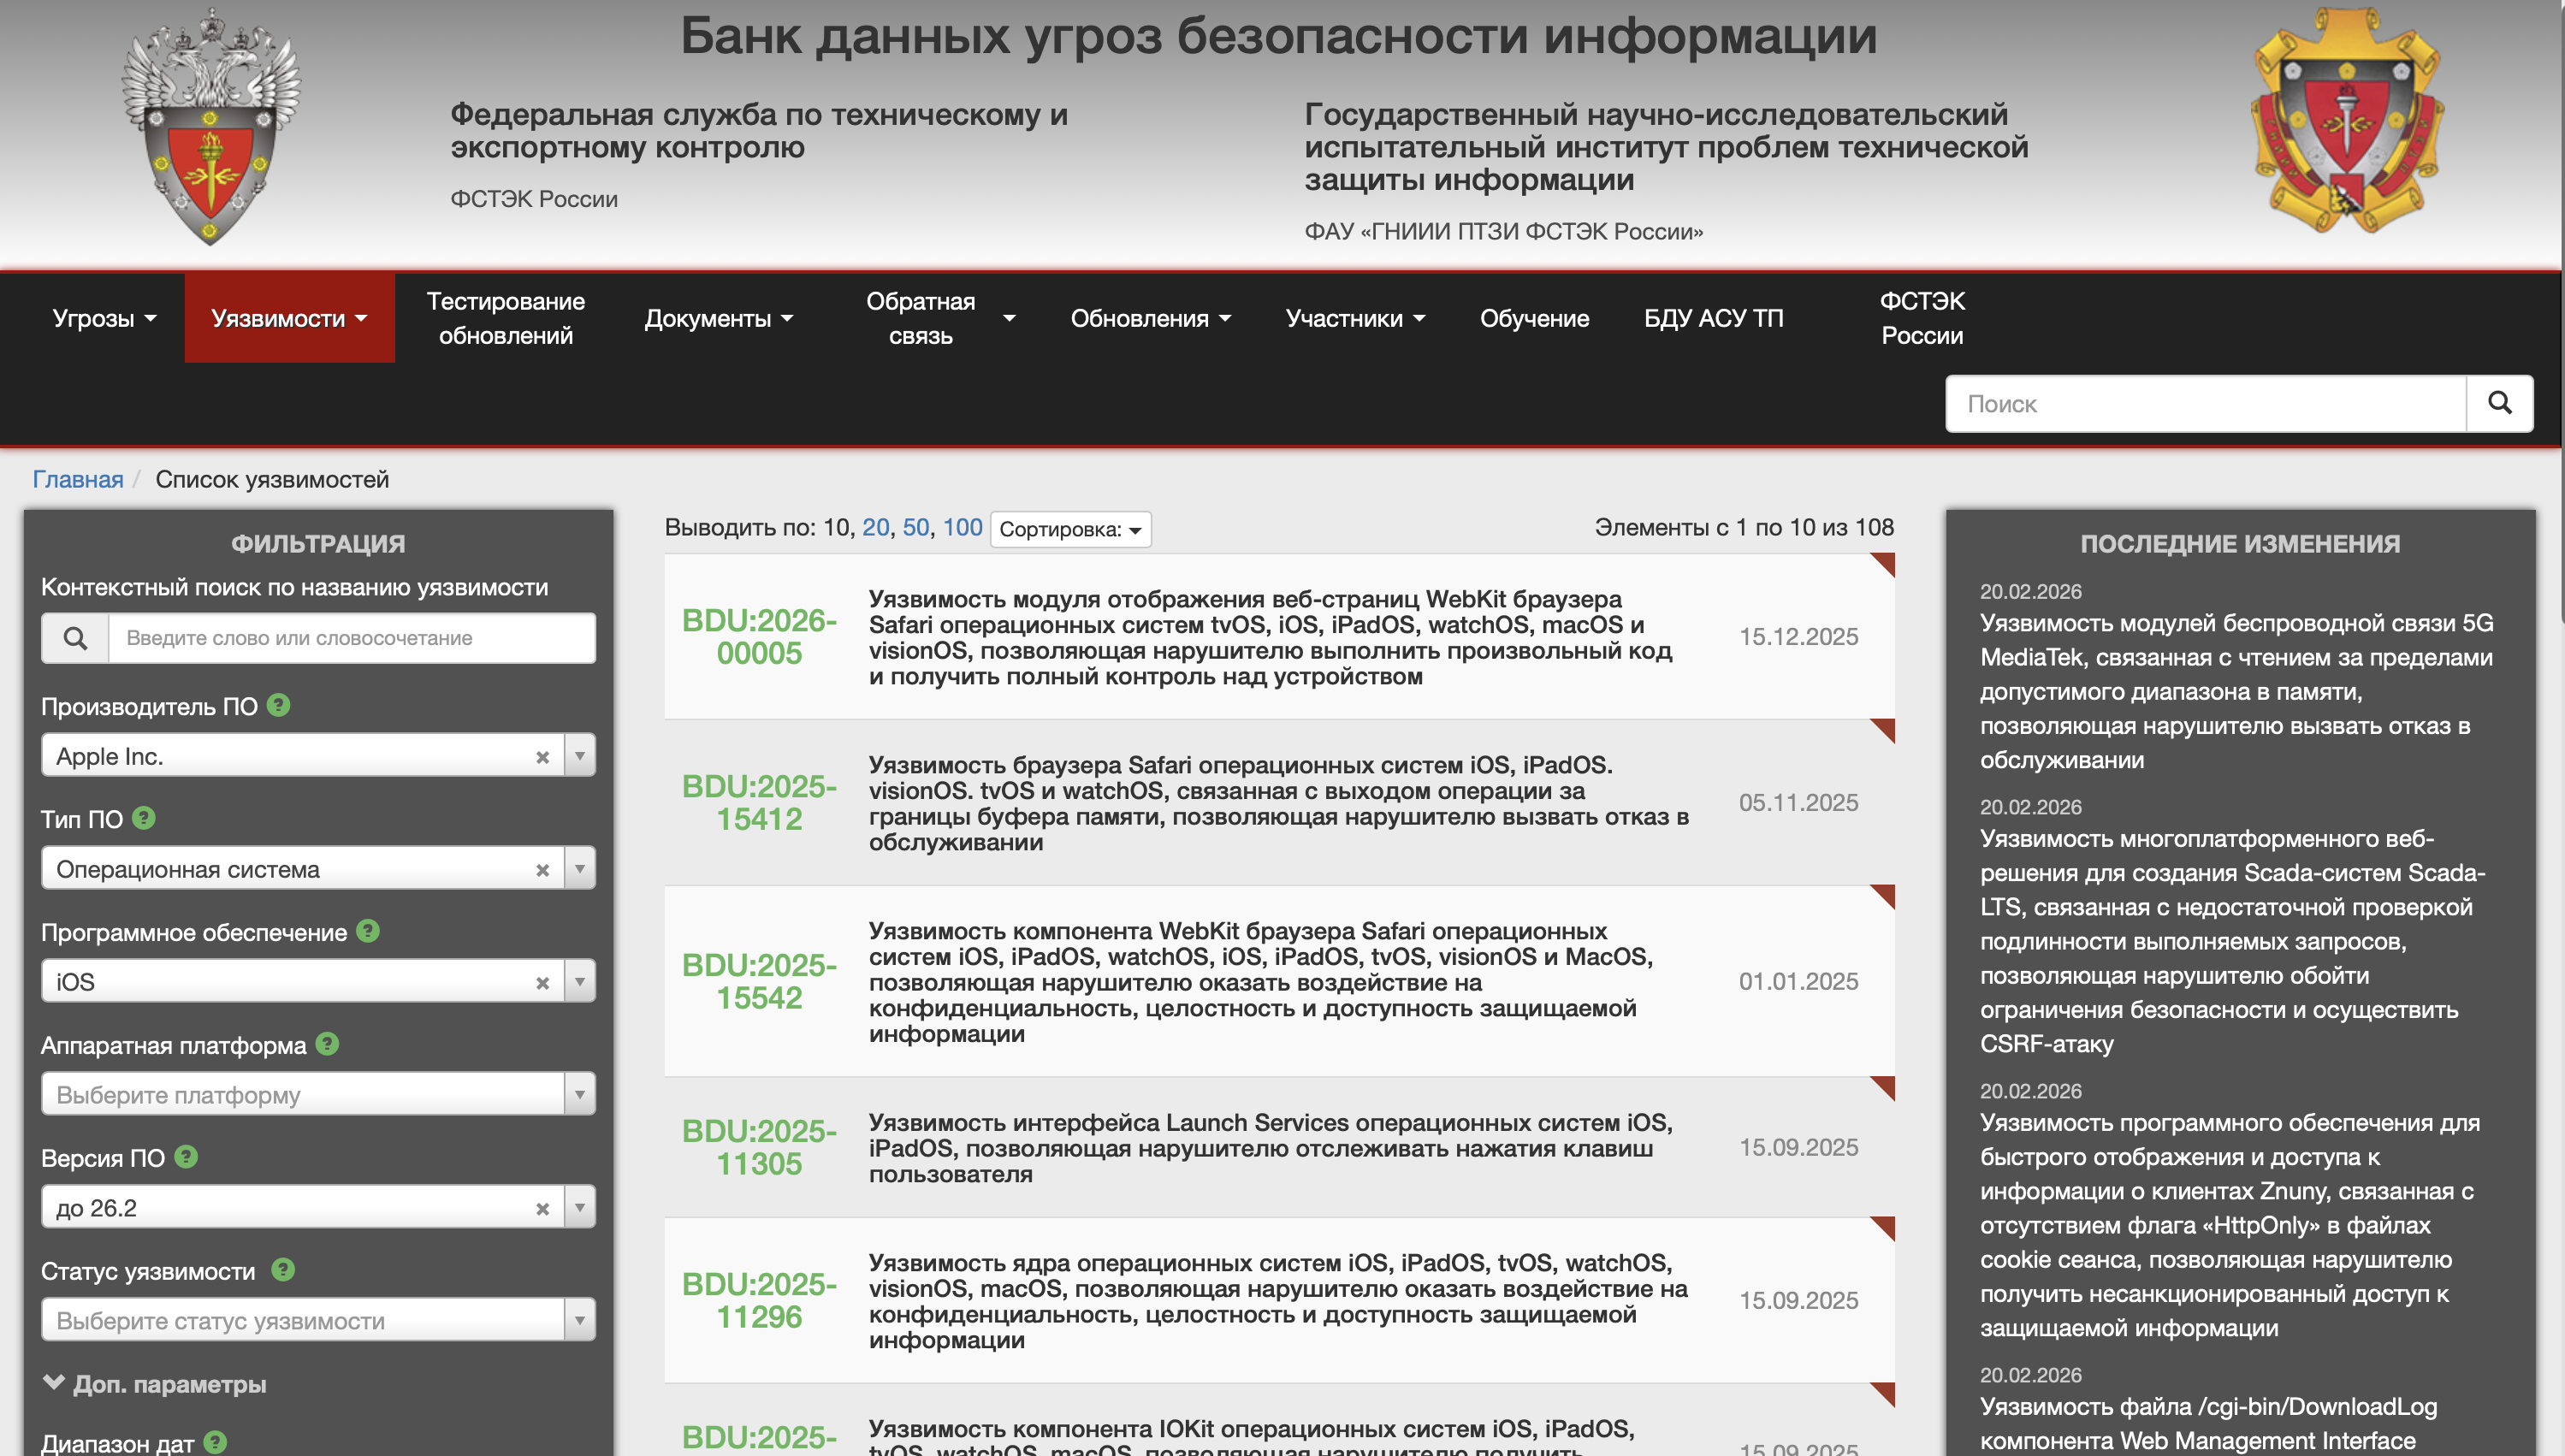
\includegraphics[width=0.60\linewidth]{img/iosfstec.png}
    \caption{Критические уязвимости в iOS}
    \label{fig:iosfstec}
\end{figure}

Возьмем первые две из отсортированных по критичности:

\begin{itemize}
    \item BDU:2026-00005;
    \item BDU:2025-15412.
\end{itemize}

BDU:2026-00005, позволяет злоумышленнику, выполнить произвольный код и получить полный контроль над устройством,
а BDU:2025-15412, связанна с выходом операции за границы буфера памяти, которая может позволить злоумышленнику вызвать отказ в обслуживании.

Более подробное описание двух уязвимостей представлены на рисунке \ref{fig:fsteciosfull1}, и \ref{fig:fsteciosfull2}.

\begin{figure}[H]
    \centering
    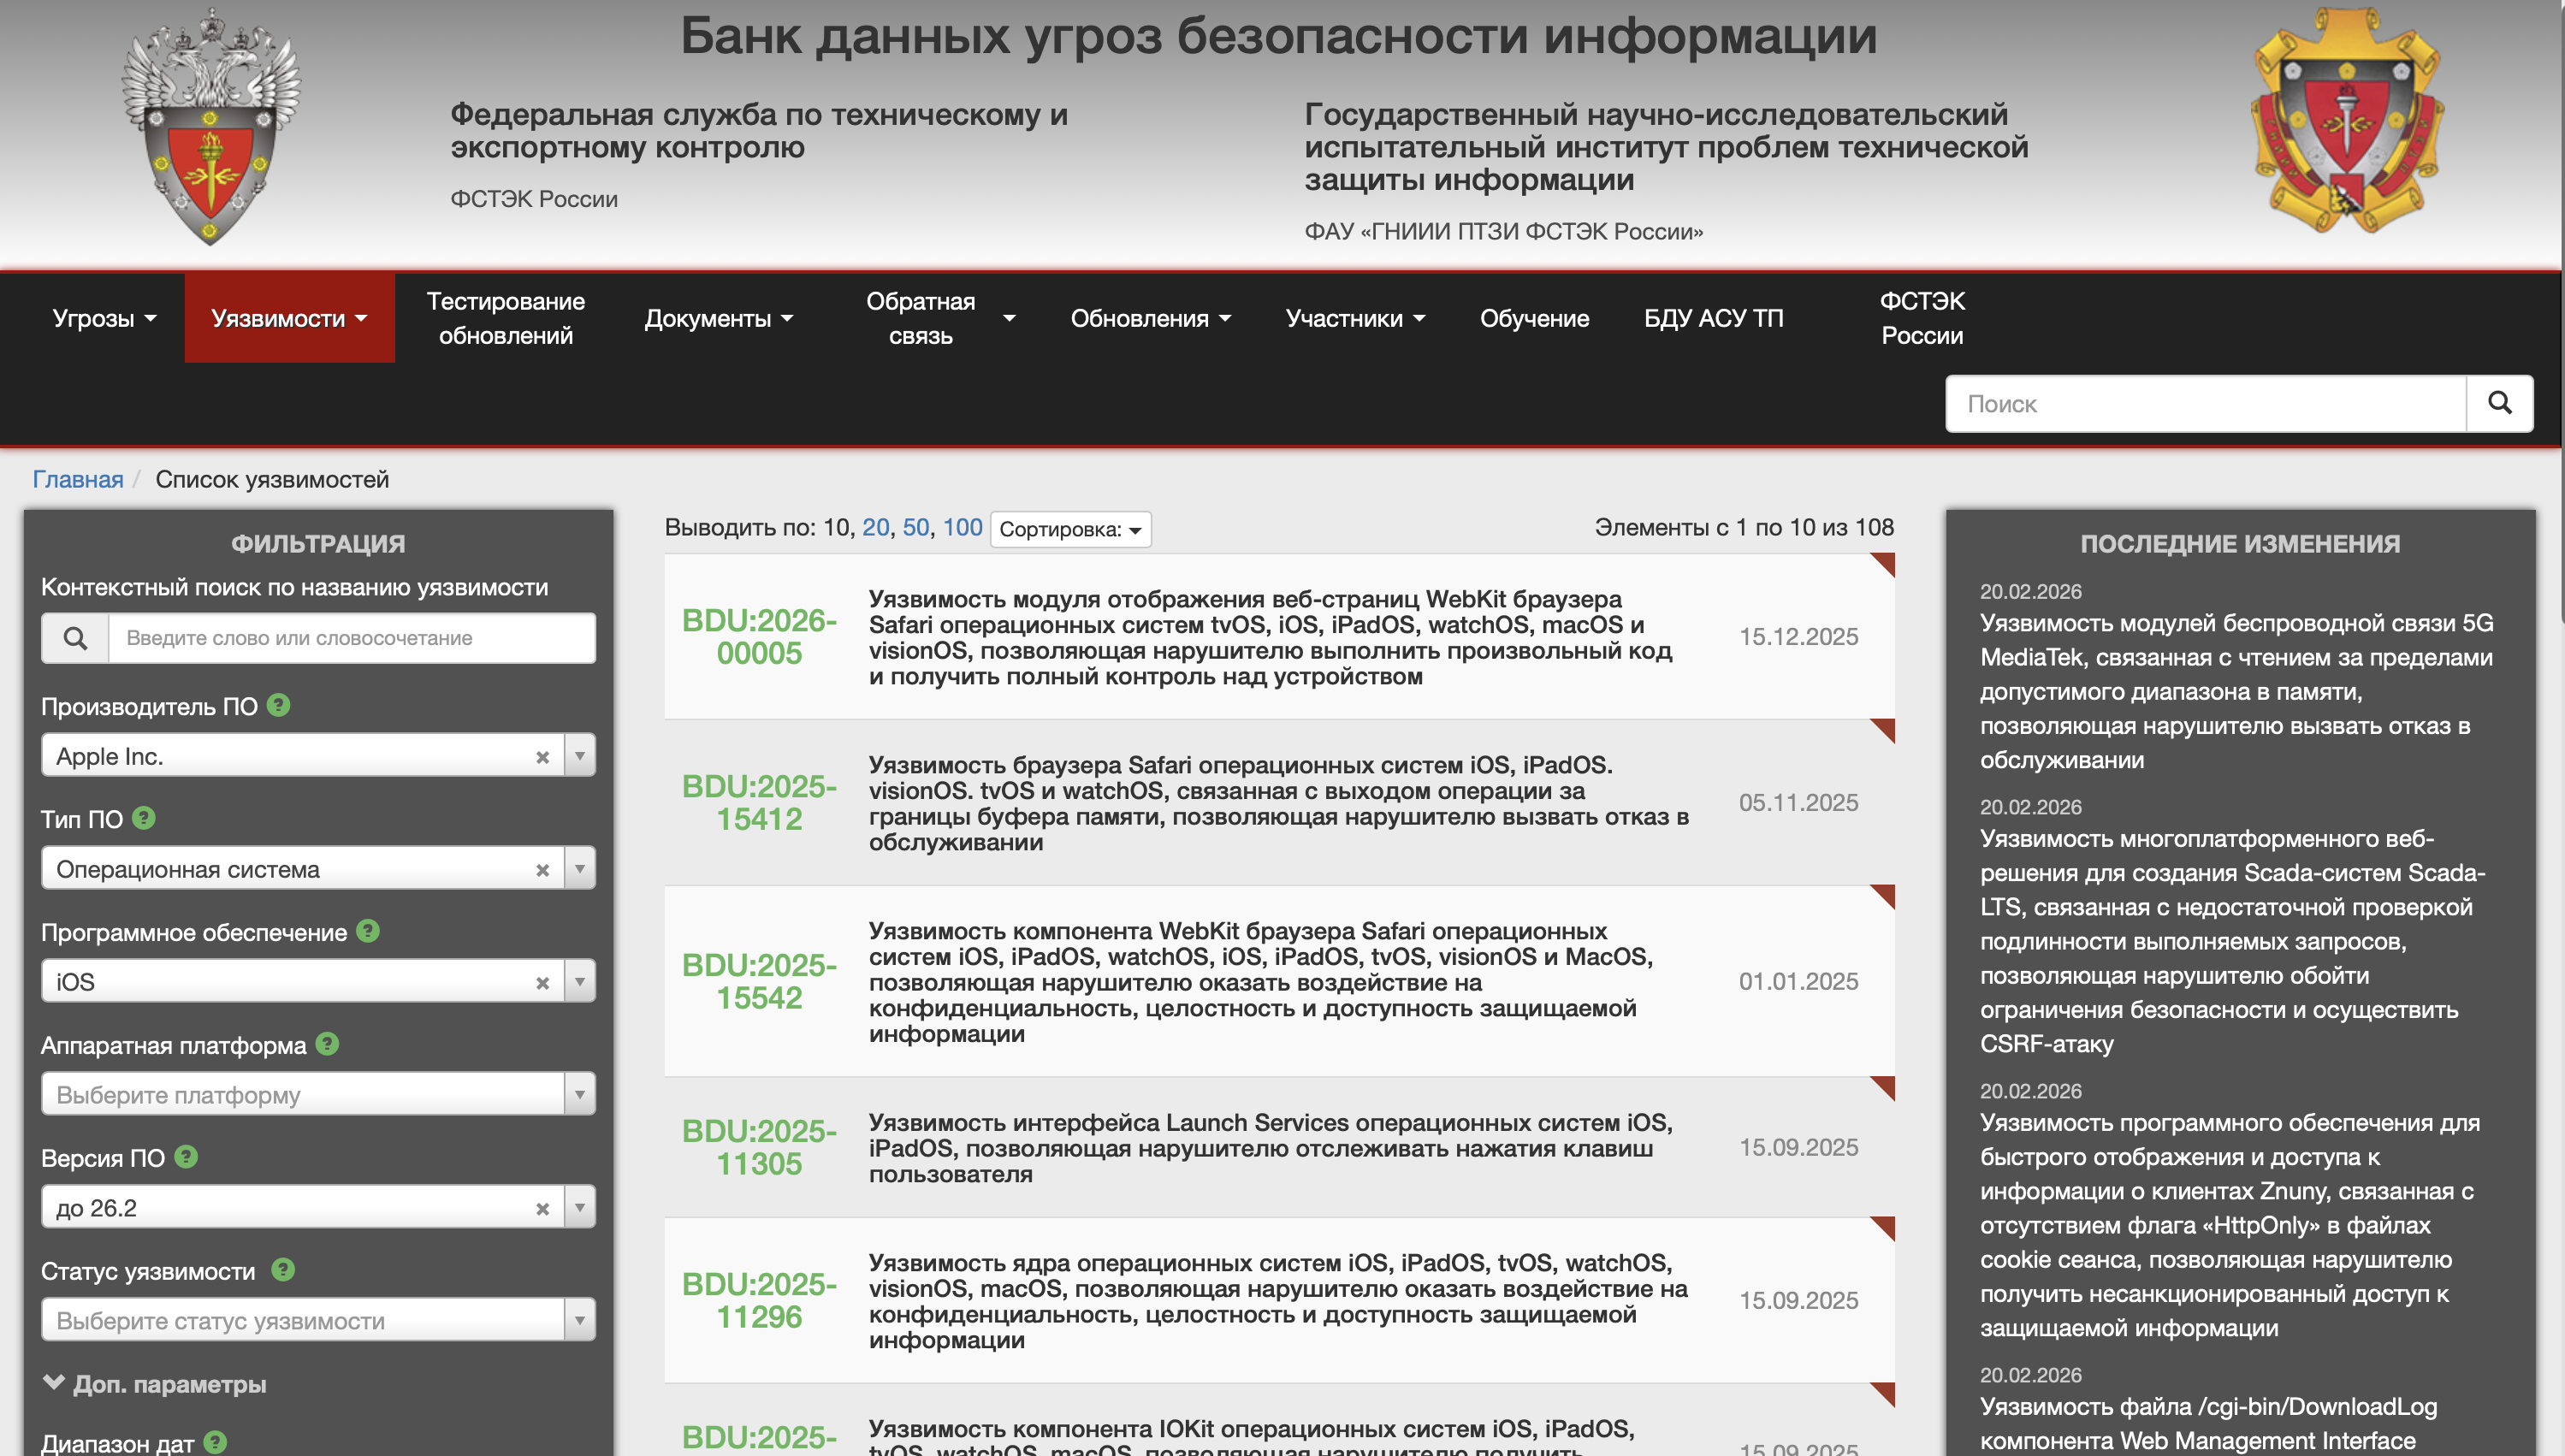
\includegraphics[width=0.60\linewidth]{img/iosfstec.png}
    \caption{Уязвимость критического уровня BDU:2026-00005}
    \label{fig:fsteciosfull1}
\end{figure}

\begin{figure}[H]
    \centering
    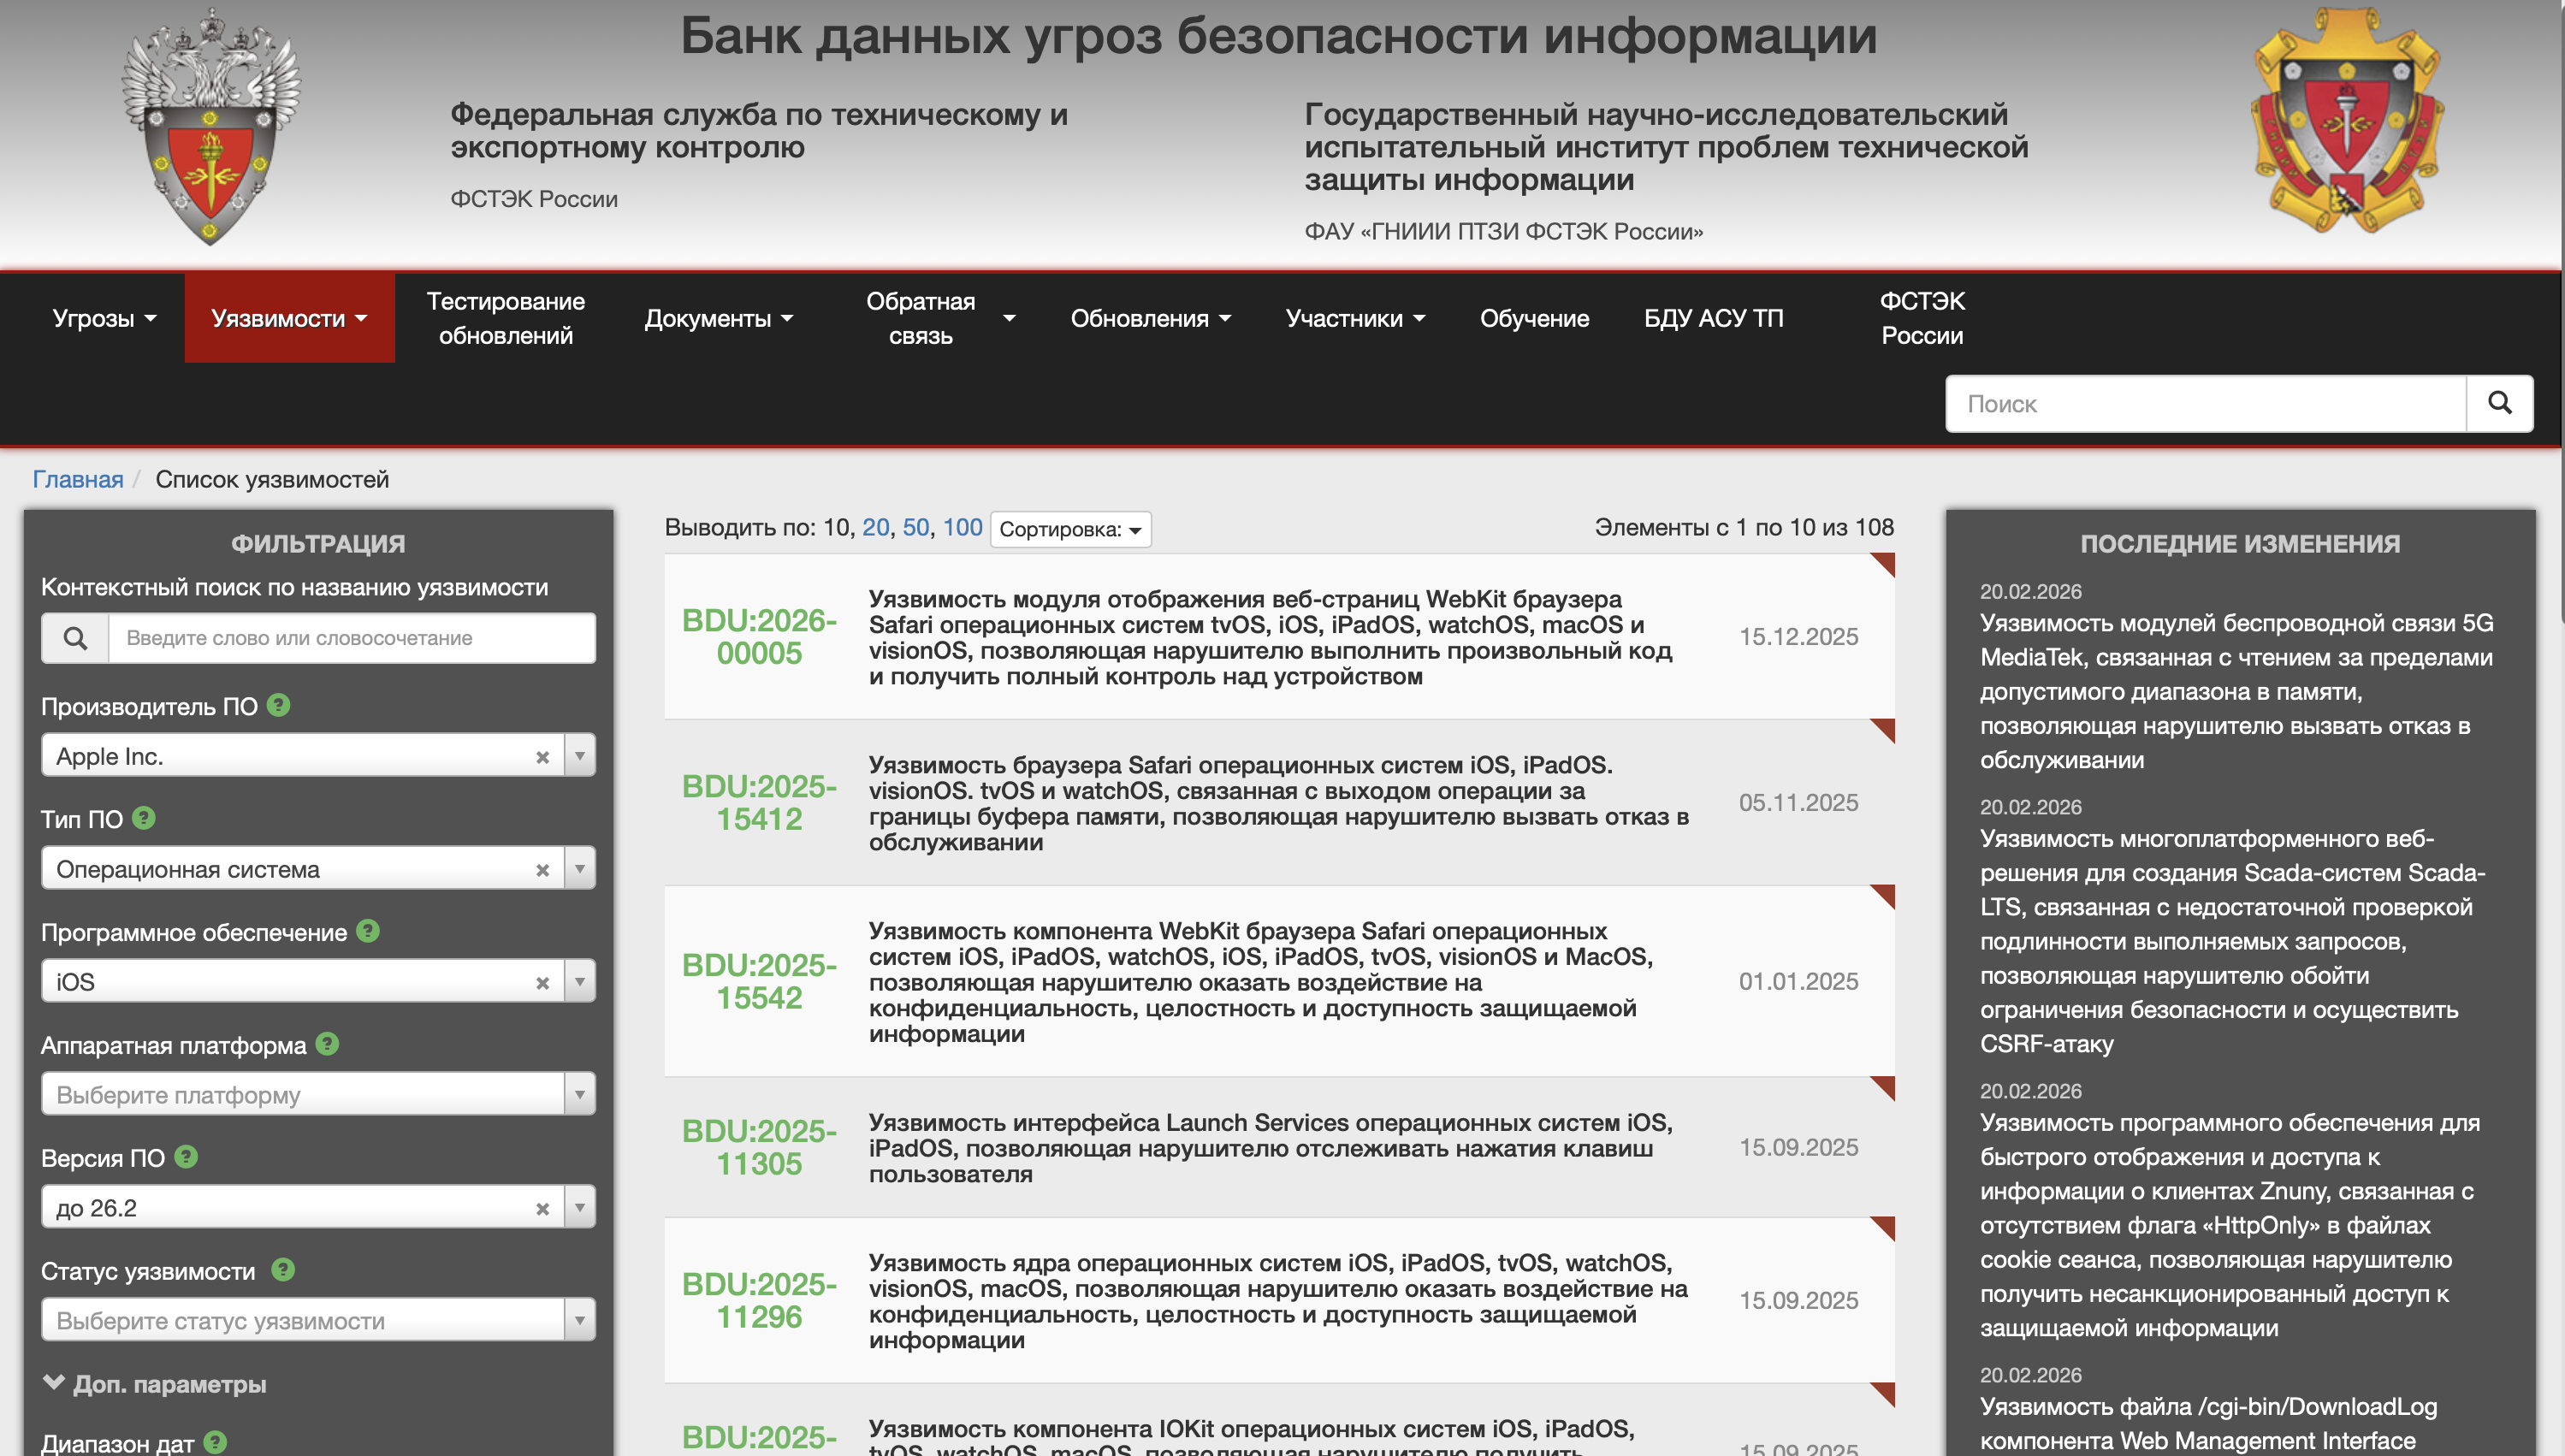
\includegraphics[width=0.60\linewidth]{img/iosfstec.png}
    \caption{Уязвимость критического уровня BDU:2025-15412}
    \label{fig:fsteciosfull2}
\end{figure}

Так же опишем их базовые вектора уязвимостей:

\begin{itemize}
    \item BDU:2026-00005: \begin{itemize}
        \item CVSS 2.0: AV:N/AC:L/Au:N/C:C/I:C/A:C
        \item CVSS 3.0: AV:N/AC:L/PR:N/UI:R/S:U/C:H/I:H/A:H
        \item CVSS 4.0: - 
    \end{itemize}
    \item BDU:2025-15412: \begin{itemize}
        \item CVSS 2.0: AV:N/AC:L/Au:N/C:C/I:C/A:C
        \item CVSS 3.0: AV:N/AC:L/PR:N/UI:R/S:U/C:H/I:H/A:H
        \item CVSS 4.0: - 
    \end{itemize}
\end{itemize}

Вектора полностью идентичны, их можно описать едино:

\textbf{CVSS 2.0: AV - способ получения доступа: N - сетевой/ AC - сложность получения доступа: L - низкая/
Au - аутентификация: N - не требуется/ C - влияние на конфиденциальность: C - полное/ I - влияние
на целостность: C - полное/ A - влияние на доступность: C - полное.}

\emph{То есть это сетевой способ получения доступа с низкой сложностью, без аутентификации с влиянием на конфиденциальность, целостность и доступность.}

\textbf{CVSS 3.0: AV - вектор атаки: N - сетевой/ AC - сложность атаки: L - низкая/ PR - уровень привелегий: N - не требуется/ UI - взаимодействие с пользователем: R - требуется/ S - влияние на другие компоненты:
U - не оказывает/ C - влияние на конфиденциальность: H - высокое/ I - влияние
на целостность: H - высокое/ A - влияние на доступность: H - высокое.}

\emph{То есть сетевая атака с низкой сложностью, без требования привелегий, со взаимодействием с пользователем, не влияющий на другие компоненты, высоко влияющий на конфиденциальность, целостность и доступность.}

\subsection*{Заключение лабораторной работы №1}
\addcontentsline{toc}{subsection}{Заключение лабораторной работы №1}
В ходе выполнения лабораторной работы №1, был изучен Банк угроз ФСТЭК, в котором были выявлины уязвимости для имеющихся операционных систем ноутбука (macOS) и смартфона (iOS). 
В ходе исследования уязвимостей, было выявлено, что операционная система macOS, достаточно хорошо защищена, так как были найденны всего две уязвимости среднего и одна низкого уровня. 
Уязвимости были связаны с модулем WebKit, который мог предоставить частичный доступ к информации. 

Так же было выявлено, что iOS, недостаточно защищенная операционная система, были выявлены критические уязвимости, связанные с полным нарушением безопасности информации, а именно влияние на конфиденциальность, целостность и доступность.
Одна из уязвимостей (относительно новая), была в том, что злоумышленник мог получить полный доступ к устройству, другая же, уязвимостей была связана с утечкой памяти, что позволяло злоумышленнику вызвать отказ в обслуживании.

\addcontentsline{toc}{subsection}{Список источников для лабораторной работы №1}

\begin{thebibliography}{99}
\bibitem{bdu}
ФСТЭК России // Банк данных угроз безопасности информации URL: \url{https://bdu.fstec.ru/} (дата обращения: 22.02.2026).
\end{thebibliography}

\end{document}